


\documentclass[11pt]{article}

\usepackage[top=.8in, bottom=.7in, left=.56in, right=.45in, footskip=0pt,
paperheight=14.16in,paperwidth=9.25in]{geometry}




\newcommand{\Ldown}[1]{\hspace{-2pt}\raisebox{-1pt}{{%\fontfamily{lmhh}
\fontsize{14}{11}\selectfont{}{\textnormal{#1.}}}}\hspace{3pt}}


\newcommand{\semihr}[1]{{\textcolor{orange!60!black}{\hrule width #1}}}


\usepackage{xcolor}


\usepackage{xcolor}



%\input{commands}

\newcommand{\mdash}{---}
\newcommand{\q}[1]{``#1''}
\newcommand{\br}{

}

\newcommand{\raggedRightTitle}[1]{\br{}\begin{flushleft}\textbf{#1}\end{flushleft}}

%\newcommand{\visavis}{vis-\`a-vis}


%\input{ngml/ngml-setup-commands}
%\input{ngml/ngml-sdi-commands}
%\input{ngml/ngml-deco-commands}

%\AtEndDocument{\immediate\write18{cd /home/nlevisrael/gits/ntxh/wip-sebi/ar/code/cpp/qmake-console/projects/gtagml/ngml-sdi-console; ./run-with-args.sh /home/nlevisrael/gits/ntxh/wip-sebi/gtagml/ctg/gen/ctg/ctg.gt.tex /home/nlevisrael/gits/ntxh/wip-sebi/gtagml/ctg/gen/ctg/ctg.gt.sdi.ntxh /home/nlevisrael/gits/ntxh/wip-sebi/gtagml/ctg/gen/ctg/ctg.gt.sdi-prelatex.ntxh; cd -;}}



% pmml  arff  openannotation

\usepackage[T1]{fontenc}
\usepackage{tgtermes}

\usepackage[hang,flushmargin]{footmisc}

\usepackage{titlesec}

\titlespacing*{\section}
{0pt}{4ex plus 1ex minus .5ex}{.1ex plus .2ex}

%\usepackage{titlesec}

\titleformat{\section}
  {\normalfont\Large\bfseries}   % The style of the section title
  {}                             % a prefix
  {0pt}                          % How much space exists between the prefix and the title
  {} 


%\usepackage{mathptmx}

\usepackage{eso-pic}

\AddToShipoutPictureBG{%

\colorlet{redbl}{red!40!magenta}
\colorlet{yelbl}{yellow!60!magenta}

\colorlet{redblg}{redbl!30!black}

\ifnum\value{page}>66{
\AtTextLowerLeft{\raisebox{-21pt}{\hspace{-15pt}\fontfamily{qtm}\fontsize{10}{11}\fontseries{b}\selectfont{}{\colorbox{yelbl!7}{\textcolor{redblg!70}{PLEASE SEE OUR SOFTWARE DEMO VIDEOS: \href{http://www.lingtechsys.com/videos/qmt-composite.mkv}{GIS},
\href{http://www.lingtechsys.com/videos/dhax-composite.mkv}{360\textdegree{} photography}, and \href{http://www.lingtechsys.com/videos/xcsd-composite.mkv}{image processing}.}}}}}
}\fi
}


%\setlength\parindent{0pt}

\AddToShipoutPictureBG{%

\ifnum\value{page}>1{
\AtTextUpperLeft{
\makebox[23.1cm][r]{
\raisebox{-.6cm}{%
{\transparent{0.3}{\includegraphics[width=0.19\textwidth]{e-logo.png}}	}} } }
}\fi
}

\AddToShipoutPicture{%
{
 {\color{blGreen!70!red}\transparent{0.9}{\put(0,0){\rule{3pt}{\paperheight}}}}%
 {\color{darkRed!70!purple}\transparent{1}\put(3,0){{\rule{4pt}{\paperheight}}}}
% {\color{logoPeach!80!cyan}\transparent{0.5}{\put(0,700){\rule{1cm}{.6cm}}}}%
% {\color{darkRed!60!cyan}\transparent{0.7}\put(0,706){{\rule{1cm}{.6cm}}}}
% \put(18,726){\thepage}
% \transparent{0.8}
}
}

%\AddToShipoutPicture{%
%\ifnum\value{page}=1
%\put(247.5,988){%
%	\transparent{0.7}{
%		
\includegraphics[width=0.4\textwidth]{logo.png}}}
%\fi
%}	


\AddToShipoutPictureBG{%
\ifnum\value{page}=14

\put(7,678){
	\transparent{1}{
		\includegraphics[angle=0.5,origin=c,width=0.4\textwidth]{pm/1a.jpg}}}


\put(241,698){
	\transparent{1}{
		\includegraphics[angle=0,origin=c,width=0.31\textwidth,
trim=0 14mm 0 10mm, clip]{pm/7a.png}}}


\put(6,492){
	\transparent{1}{
		\includegraphics[angle=-0.5,origin=c,width=0.4\textwidth]{pm/5a.png}}}


\put(452,712){
	\transparent{1}{
		\includegraphics[angle=-1,origin=c,width=0.3\textwidth]{pm/2a.png}}}



\put(442,681){
	\transparent{1}{
		\includegraphics[angle=0,origin=c,width=0.18\textwidth]{pm/8a.png}}}


%\put(412,680){
%	\transparent{1}{
%		\includegraphics[angle=2.5,origin=c,width=0.2\textwidth]{pm/8.png}}}


\put(402,487){
	\transparent{1}{
		\includegraphics[angle=-1,origin=c,width=0.45\textwidth]{pm/3a.jpg}}}

\fi
}	




%\pagestyle{empty} % no page number
%\parskip 7.2pt    % space between paragraphs
%\parindent 12pt   % indent for new paragraph
%\textwidth 4.5in  % width of text
%\columnsep 0.8in  % separation between columns

%\setlength{\footskip}{-3pt}

%\usepackage[paperheight=15in,paperwidth=8.5in]{geometry}
%\geometry{left=.65in,top=.65in,right=.45in,bottom=1.25in} %margins

%\renewcommand{\thepage}{\raisebox{2pt}{\arabic{page}}}

\renewcommand{\footnoterule}{%
	\kern -3pt
	\hrule width .92\textwidth height .5pt
	\kern 10pt
}


\usepackage[hyphens]{url}
\newcommand{\biburl}[1]{ {\fontfamily{gar}\selectfont{\textcolor[rgb]{.2,.6,0}%
{\scriptsize {\url{#1}}}}}}

\newcommand{\bhref}[1]{\href{#1}{#1}}



%\linespread{1.3}

\newcommand{\sectsp}{\vspace{12pt}}

\usepackage{graphicx}
\usepackage{color,framed}

\usepackage{textcomp}

\usepackage{float}

\usepackage{mdframed}


\usepackage{setspace}

\usepackage{xcolor}

\usepackage[hyphenbreaks]{breakurl}
\usepackage[hyphens]{url}

%\usepackage{hyperref}

\colorlet{blCyan}{cyan!50!blue}

\definecolor{darkRed}{rgb}{.2,.0,.1}


\definecolor{blGreen}{rgb}{.2,.7,.3}

\definecolor{darkBlGreen}{rgb}{.1,.3,.2}

\definecolor{oldBlColor}{rgb}{.2,.7,.3}

\definecolor{blColor}{rgb}{.1,.3,.2}

\definecolor{elColor}{rgb}{.2,.1,0}
\definecolor{flColor}{rgb}{0.7,0.3,0.3}

\definecolor{logoOrange}{RGB}{108, 18, 30}
\definecolor{logoGreen}{RGB}{85, 153, 89}
\definecolor{logoPurple}{RGB}{200, 208, 30}

\definecolor{logoBlue}{RGB}{4, 2, 25}
\definecolor{logoPeach}{RGB}{255, 159, 102}
\definecolor{logoCyan}{RGB}{66, 206, 244}
\definecolor{logoRed}{rgb}{.3,0,0}

\newcommand{\colorq}[1]{{\color{logoOrange!70!black}{\q{\small\textbf{#1}}}}}

\let\qq\q

\definecolor{inOne}{rgb}{0.122, 0.435, 0.698}% Rule colour
\definecolor{inTwo}{rgb}{0.122, 0.698, 0.435}% Rule colour

\definecolor{outOne}{rgb}{0.435, 0.698, 0.122}% Rule colour
\definecolor{outTwo}{rgb}{0.698, 0.435, 0.122}% Rule colour

\colorlet{linkcolor}{flColor!60!red}




\usepackage[many]{tcolorbox}% http://ctan.org/pkg/tcolorbox

\usepackage{transparent}

\newlength{\bsep}
\setlength{\bsep}{-1pt}
\let\xbibitem\bibitem
\renewcommand{\bibitem}[2]{\vspace{\bsep}\xbibitem{#1}{#2}}

\newenvironment{cframed}{\begin{mdframed}[linecolor=logoPeach,linewidth=0.4mm]}{\end{mdframed}}

\newenvironment{ccframed}{\begin{mdframed}[backgroundcolor=logoGreen!5,linecolor=logoCyan!50!black,linewidth=0.4mm]}{\end{mdframed}}

\usepackage{aurical}
\usepackage[T1]{fontenc}

\usepackage{relsize}

\newcommand{\bref}[1]{\hspace*{1pt}\textbf{\ref{#1}}}

\newcommand{\dashsep}{--\hspace*{5pt}}

\newcommand{\pseudoIndent}{

\vspace{2pt}\hspace*{6.5pt}}

\usepackage{titlesec}

\titlespacing*{\subsection}
{0pt}{5ex plus 1ex minus .2ex}{0.5ex plus .2ex}


%\titlespacing*{\section}
%{0pt}{3.5ex plus 1ex minus .2ex}{1ex plus .2ex}

%
\newcommand{\deconum}[1]{{\protect\raisebox{-1pt}{{\LARGE #1}}}}

\newcommand{\visavis}{vis-\`a-vis}

\newcommand{\VersatileUX}{{\color{red!85!black}{\Fontauri Versatile}}%
{{\fontfamily{qhv}\selectfont\smaller UX}}}

\newcommand{\NDPCloud}{{\color{red!15!black}%
{\fontfamily{qhv}\selectfont {\smaller NDP C{\smaller LOUD}}}}}

\newcommand{\MThreeK}{{\color{blGreen!45!black}%
{\fontfamily{qhv}\fontsize{10}{8}\selectfont {M3K}}}}


\newcommand{\lfNDPCloud}{{\color{red!15!black}%
{\fontfamily{qhv}\selectfont N{\smaller DP C{\smaller LOUD}}}}}

\newcommand{\textds}[1]{{\fontfamily{lmdh}\selectfont{%
\raisebox{-1pt}{#1}}}}

\newcommand{\dsC}{{\textds{ds}{\fontfamily{qhv}\selectfont \raisebox{-1pt}
{\color{red!15!black}{C}}}}}

\definecolor{tcolor}{RGB}{24,52,61}

\newcommand{\CCpp}{\resizebox{!}{6.5pt}{\AcronymText{C}}/\Cpp{}}
\newcommand{\NoSQL}{\resizebox{!}{6.5pt}{\AcronymText{NoSQL}}}
\newcommand{\SQL}{\resizebox{!}{6.5pt}{\AcronymText{SQL}}}

\newcommand{\NCBI}{\resizebox{!}{6.5pt}{\AcronymText{NCBI}}}
\newcommand{\BioNetGen}{\resizebox{!}{6.5pt}{\AcronymText{BioNetGen}}}
\newcommand{\BNGL}{\resizebox{!}{6.5pt}{\AcronymText{BNGL}}}

\newcommand{\GML}{\resizebox{!}{6.5pt}{\AcronymText{GML}}}

\newcommand{\GIS}{\resizebox{!}{6.5pt}{\AcronymText{GIS}}}
\newcommand{\ACRIS}{\resizebox{!}{6.5pt}{\AcronymText{ACRIS}}}
\newcommand{\HPD}{\resizebox{!}{6.5pt}{\AcronymText{HPD}}}


\newcommand{\HTXN}{\resizebox{!}{6.5pt}{\AcronymText{HTXN}}}

\newcommand{\TDM}{\resizebox{!}{6.5pt}{\AcronymText{TDM}}}

\newcommand{\lHTXN}{\resizebox{!}{7.5pt}{\AcronymText{H}}%
\resizebox{!}{6.5pt}{\AcronymText{TXN}}}

\newcommand{\lsHTXN}{\resizebox{!}{9.5pt}{\AcronymText{\textcolor{tcolor}{HTXN}}}}

\newcommand{\LAF}{\resizebox{!}{6.5pt}{\AcronymText{LAF}}}

\newcommand{\UDpipe}{\resizebox{!}{6.5pt}{\AcronymText{UDpipe}}}

\newcommand{\C}{\resizebox{!}{6.5pt}{\AcronymText{C}}}

\newcommand{\TME}{\resizebox{!}{6.5pt}{\AcronymText{TME}}}

\newcommand{\TwoD}{\resizebox{!}{6.5pt}{\AcronymText{2D}}}




\usepackage{mdframed}

\newcommand{\cframedboxpanda}[1]{\begin{mdframed}[linecolor=yellow!70!blue,linewidth=0.4mm]#1\end{mdframed}}





\newcommand{\libSBML}{\resizebox{!}{6.5pt}{\AcronymText{libSBML}}}


\newcommand{\PVD}{\resizebox{!}{6.5pt}{\AcronymText{PVD}}}


\newcommand{\SDK}{\resizebox{!}{6.5pt}{\AcronymText{SDK}}}
\newcommand{\NLP}{\resizebox{!}{6.5pt}{\AcronymText{NLP}}}


\newcommand{\PDF}{\resizebox{!}{6.5pt}{\AcronymText{PDF}}}
\newcommand{\TEI}{\resizebox{!}{7.5pt}{\AcronymText{TE{\hspace*{.5pt}I}}}}
\newcommand{\SSML}{\resizebox{!}{7.5pt}{\AcronymText{SSML}}}
\newcommand{\ToBI}{\resizebox{!}{7.5pt}{\AcronymText{ToBI}}}

\newcommand{\MMBioS}{\resizebox{!}{6.5pt}{\AcronymText{MMBioS}}}

\newcommand{\VTK}{\resizebox{!}{6.5pt}{\AcronymText{VTK}}}


\newcommand{\AXF}{\resizebox{!}{6.5pt}{\AcronymText{AXF}}}

\newcommand{\HyperGraphDB}{\resizebox{!}{6.5pt}{\AcronymText{HyperGraphDB}}}


\newcommand{\lAXF}{\resizebox{!}{7.5pt}{\AcronymText{A}}%
\resizebox{!}{6.5pt}{\AcronymText{XF}}}


\newcommand{\lsAXF}{\resizebox{!}{8.5pt}{\AcronymText{AXF}}}

\newcommand{\AXFD}{\resizebox{!}{6.5pt}{\AcronymText{AXFD}}}

\newcommand{\lAXFD}{\resizebox{!}{7.5pt}{\AcronymText{A}}%
\resizebox{!}{6.5pt}{\AcronymText{XFD}}}


\newcommand{\IJST}{\resizebox{!}{6.5pt}{\AcronymText{IJST}}}

\newcommand{\BioC}{\resizebox{!}{6.5pt}{\AcronymText{BioC}}}

\newcommand{\CoNLL}{\resizebox{!}{6.5pt}{\AcronymText{CoNLL}}}
\newcommand{\CoNLLU}{\resizebox{!}{6.5pt}{\AcronymText{CoNLL-U}}}


\newcommand{\ePub}{\resizebox{!}{6.5pt}{\AcronymText{ePub}}}

%\lsLPF

\definecolor{atcColor}{RGB}{96, 17, 12}
%\textcolor{tcolor}{

\newcommand{\ATextCClr}[1]{\textcolor{atcColor}{\textbf{#1}}}

\newcommand{\ATexttclr}[1]{\textcolor{tcolor}{\textbf{#1}}}
\newcommand{\THQL}{\resizebox{!}{6.5pt}{\ATexttclr{THQL}}}


\newcommand{\ATextbk}[1]{\textcolor{black!50!cyan}{\textbf{#1}}}


%\newcommand{\lDHOS}{\resizebox{!}{6.5pt}{\ATexttclr{D}}%
%resizebox{!}{6.5pt}{\ATexttclr{HOS}}}

\newcommand{\PGVM}{\resizebox{!}{6.5pt}{\ATexttclr{PGVM}}}
\newcommand{\lPGVM}{\resizebox{!}{6.5pt}{\ATexttclr{PGVM}}}

\newcommand{\DHOS}{\resizebox{!}{6.5pt}{\ATexttclr{DHOS}}}
\newcommand{\lDHOS}{\resizebox{!}{7.5pt}{\ATexttclr{D}}\resizebox{!}{6.5pt}{\ATexttclr{HOS}}}
\newcommand{\sDHOS}{\resizebox{!}{6.5pt}{\ATexttclr{DHOS}}}

\newcommand{\sQt}{\resizebox{!}{6.5pt}{\ATexttclr{Qt}}}

\newcommand{\sPhVM}{\resizebox{!}{6.5pt}{\ATexttclr{P\hspace{.5pt}\textit{h}\hspace*{-.5pt}VM}}}


\newcommand{\PhVM}{\resizebox{!}{6.5pt}{\ATexttclr{P\hspace{.5pt}\textit{h}\hspace*{-.5pt}VM}}}
\newcommand{\lPhVM}{\resizebox{!}{7.5pt}{\ATexttclr{P}}\resizebox{!}{6.5pt}{\ATexttclr{\hspace{1pt}\textit{h}\hspace*{-.5pt}VM}}}


\newcommand{\MOC}{\resizebox{!}{6.5pt}{\AcronymText{MOC}}}
\newcommand{\SPARQL}{\resizebox{!}{6.5pt}{\AcronymText{SPARQL}}}
\newcommand{\GraphQL}{\resizebox{!}{6.5pt}{\AcronymText{GraphQL}}}

%{}, \QML{}, \GraphQL

\newcommand{\CCi}{\resizebox{!}{6.5pt}{\ATexttclr{CCi}}}
\newcommand{\XCSD}{\resizebox{!}{6.5pt}{\ATexttclr{XCSD}}}

\newcommand{\lXCSD}{\resizebox{!}{6.5pt}{\ATexttclr{XCSD}}}
\newcommand{\lCCi}{\resizebox{!}{6.5pt}{\ATexttclr{CCi}}}

%\newcommand{\ConceptsDB}{\resizebox{!}{6.5pt}{\ATexttclr{ConceptsDB}}}
%\newcommand{\lConceptsDB}{\resizebox{!}{6.5pt}{\ATexttclr{C}}\resizebox{!}{6.5pt}%{\ATexttclr{onceptsDB}}}


\newcommand{\GIT}{\resizebox{!}{6.5pt}{\AcronymText{GIT}}}

\newcommand{\LPF}{\resizebox{!}{6.5pt}{\AcronymText{LPF}}}
\newcommand{\lLPF}{\resizebox{!}{8.5pt}{\AcronymText{LPF}}}
\newcommand{\lsLPF}{\resizebox{!}{9.5pt}{\AcronymText{LPF}}}

\makeatletter

\newcommand*\getX[1]{\expandafter\getX@i#1\@nil}

\newcommand*\getY[1]{\expandafter\getY@i#1\@nil}
\def\getX@i#1,#2\@nil{#1}
\def\getY@i#1,#2\@nil{#2}
\makeatother
	
\newcommand{\rectann}[9]{%
\path [draw=#1,draw opacity=#2,line width=#3, fill=#4, fill opacity = #5, even odd rule] %
(#6) rectangle(\getX{#6}+#7,\getY{#6}+#8)
({\getX{#6}+((#7-(#7*#9))/2)},{\getY{#6}+((#8-(#8*#9))/2)}) rectangle %
({\getX{#6}+((#7-(#7*#9))/2)+#7*#9},{\getY{#6}+((#8-(#8*#9))/2)+#8*#9});}


\definecolor{pfcolor}{RGB}{94, 54, 73}

\newcommand{\EPF}{\resizebox{!}{6.5pt}{\AcronymText{ETS{\color{pfcolor}pf}}}}
\newcommand{\lEPF}{\resizebox{!}{8.5pt}{\AcronymText{ETS{\color{pfcolor}pf}}}}
\newcommand{\lsEPF}{\resizebox{!}{9.5pt}{\AcronymText{ETS{\color{pfcolor}pf}}}}

\newcommand{\RGB}{\resizebox{!}{6.5pt}{\AcronymText{RGB}}}


\newcommand{\GRE}{\resizebox{!}{6.5pt}{\AcronymText{GRE}}}
\newcommand{\CAS}{\resizebox{!}{6.5pt}{\AcronymText{CAS}}}

\newcommand{\lMOSAIC}{%
\resizebox{!}{8pt}{\AcronymText{M}}%
\resizebox{!}{6.5pt}{\AcronymText{OSAIC}}}

\newcommand{\XML}{\resizebox{!}{6.5pt}{\AcronymText{XML}}}
\newcommand{\RDF}{\resizebox{!}{6.5pt}{\AcronymText{RDF}}}
\newcommand{\DOM}{\resizebox{!}{6.5pt}{\AcronymText{DOM}}}


\newcommand{\CWL}{\resizebox{!}{6.5pt}{\AcronymText{CWL}}}




\newcommand{\Covid}{\resizebox{!}{6.5pt}{\AcronymText{Covid-19}}}

\newcommand{\CLang}{\resizebox{!}{6.5pt}{\AcronymText{C}}}

\newcommand{\HNaN}{\resizebox{!}{6.5pt}{\AcronymText{HN%
\textsc{a}N}}}

\newcommand{\JSON}{\resizebox{!}{6.5pt}{\AcronymText{JSON}}}

\newcommand{\MeshLab}{\resizebox{!}{6.5pt}{\AcronymText{MeshLab}}}
%\newcommand{\IQmol}{\resizebox{!}{6.5pt}{\AcronymText{IQmol}}}

\newcommand{\SGML}{\resizebox{!}{6.5pt}{\AcronymText{SGML}}}

\newcommand{\ASCII}{\resizebox{!}{6.5pt}{\AcronymText{ASCII}}}



\newcommand{\JATS}{\resizebox{!}{6.5pt}{\AcronymText{JATS}}}


\newcommand{\SDI}{\resizebox{!}{6.5pt}{\AcronymText{SDI}}}
\newcommand{\SDIV}{\resizebox{!}{6.5pt}{\AcronymText{SDIV}}}

\newcommand{\VXL}{\resizebox{!}{6.5pt}{\AcronymText{VXL}}}
\newcommand{\IQmol}{\resizebox{!}{6.5pt}{\AcronymText{IQmol}}}




\newcommand{\VM}{\resizebox{!}{6.5pt}{\AcronymText{VM}}}
\newcommand{\sVM}{\resizebox{!}{6.5pt}{\AcronymText{VM}}}


\newcommand{\IDE}{\resizebox{!}{6.5pt}{\AcronymText{IDE}}}


\newcommand{\OS}{\resizebox{!}{6.5pt}{\AcronymText{OS}}}

\newcommand{\FAIR}{\resizebox{!}{6.5pt}{\AcronymText{FAIR}}}
\newcommand{\FAIRsharing}{\resizebox{!}{6.5pt}{\AcronymText{FAIR}}\hspace*{1pt}\resizebox{!}{8pt}{sharing}}

\newcommand{\Python}{\resizebox{!}{6.5pt}{\AcronymText{Python}}}
\newcommand{\RPC}{\resizebox{!}{6.5pt}{\AcronymText{RPC}}}

\newcommand{\Java}{\resizebox{!}{6.5pt}{\AcronymText{Java}}}

\newcommand{\sBioNetGen}{\resizebox{!}{6.5pt}{\AcronymText{BioNetGen}}}
\newcommand{\sUI}{\resizebox{!}{6.5pt}{\AcronymText{UI}}}
\newcommand{\sAPOLLO}{\resizebox{!}{6.5pt}{\AcronymText{APOLLO}}}
\newcommand{\sSDK}{\resizebox{!}{6.5pt}{\AcronymText{SDK}}}
\newcommand{\sGUI}{\resizebox{!}{6.5pt}{\AcronymText{GUI}}}
\newcommand{\sAPI}{\resizebox{!}{6.5pt}{\AcronymText{API}}}




\newcommand{\QNetworkManager}{\resizebox{!}{6.5pt}{\AcronymText{QNetworkManager}}}
\newcommand{\QTextDocument}{\resizebox{!}{6.5pt}{\AcronymText{QTextDocument}}}

\newcommand{\QWebEngineView}{\resizebox{!}{6.5pt}{\AcronymText{QWebEngineView}}}

\newcommand{\HTTP}{\resizebox{!}{6.5pt}{\AcronymText{HTTP}}}


\newcommand{\lAcronymTextNC}[2]{{\fontfamily{fvs}\selectfont {\Large{#1}}{\large{#2}}}}

\newcommand{\AcronymTextNC}[1]{{\fontfamily{fvs}\selectfont {\large #1}}}



\colorlet{orr}{orange!60!red}

\colorlet{orb}{green!60!blue}
\colorlet{orbb}{green!30!blue}



\newcommand{\usstitle}[1]{\vspace{.4em}\raisebox{-1.2em}{{\fontfamily{gar}\fontsize{12}{14}%
\fontseries{sb}\selectfont{{\textcolor{orbb!65!black}{#1}}}}}}}


\newcommand{\sstitle}[1]{\vspace{1em}\raisebox{-1.2em}{{\fontfamily{gar}\fontsize{12}{14}%
\fontseries{sb}\selectfont{{\textcolor{orbb!65!black}{#1}}}}}}}

\newcommand{\DaSemio}{{\fontfamily{fvs}\fontsize{9}{14}%
\selectfont{\textbf{\textcolor{orb!75!black}{Da\resizebox{6.5pt}{!}{S}emio}}}}}}


\newcommand{\lDaSemio}{{\fontfamily{fvs}\fontsize{9}{14}%
\selectfont{\textbf{\textcolor{orb!75!black}{\resizebox{9pt}{!}{D}aSemio}}}}}}


%\newcommand{\DaSemio}{DaSemio}



\newcommand{\textscci}[1]{{\color{orr!35!black}{{%
						\fontfamily{Cabin-TLF}\fontseries{b}\selectfont{\textit{\scriptsize{#1}}}}}}}


\newcommand{\textscc}[1]{{\color{orr!35!black}{{%
						\fontfamily{Cabin-TLF}\fontseries{b}\selectfont{\textsc{\scriptsize{#1}}}}}}}


\newcommand{\textsccserif}[1]{{\color{orr!35!black}{{%
				\scriptsize{\textbf{#1}}}}}}


\newcommand{\iEPF}{\resizebox{!}{6.5pt}{\textsccserif{%
\textit{ETSpf}}}}

\newcommand{\iSDI}{\resizebox{!}{6.5pt}{\textsccserif{%
\textit{SDI}}}}

\newcommand{\iHTXN}{\resizebox{!}{6.5pt}{\textsccserif{%
\textit{HTXN}}}}




\newcommand{\AcronymText}[1]{{\textscc{#1}}}
\newcommand{\iAcronymText}[1]{{\textscci{#1}}}

\newcommand{\AcronymTextser}[1]{{\textsccserif{#1}}}


\newcommand{\mAcronymText}[1]{{\textscc{\normalsize{#1}}}}

\newcommand{\FASTA}{{\resizebox{!}{6.5pt}{\AcronymText{FASTA}}}}
\newcommand{\SRA}{{\resizebox{!}{6.5pt}{\AcronymText{SRA}}}}
\newcommand{\DNA}{{\resizebox{!}{6.5pt}{\AcronymText{DNA}}}}
\newcommand{\MAP}{{\resizebox{!}{6.5pt}{\AcronymText{MAP}}}}
\newcommand{\EPS}{{\resizebox{!}{6.5pt}{\AcronymText{EPS}}}}

\newcommand{\CSV}{{\resizebox{!}{6.5pt}{\AcronymText{CSV}}}}

%\newcommand{\PDB}{{\resizebox{!}{6.5pt}{\AcronymText{PDB}}}}


\newcommand{\APOLLO}{{\resizebox{!}{6.5pt}{\AcronymText{APOLLO}}}}
\newcommand{\GDC}{{\resizebox{!}{6.5pt}{\AcronymText{GDC}}}}
\newcommand{\TCIA}{{\resizebox{!}{6.5pt}{\AcronymText{TCIA}}}}
\newcommand{\CPTAC}{{\resizebox{!}{6.5pt}{\AcronymText{CPTAC}}}}





\newcommand{\XOCS}{{\resizebox{!}{6.5pt}{\AcronymText{XOCS}}}}


\newcommand{\cytoLib}{{\resizebox{!}{6.5pt}{\AcronymText{cytoLib}}}}
\newcommand{\CaPTk}{{\resizebox{!}{6.5pt}{\AcronymText{CaPTk}}}}
\newcommand{\DCMTK}{{\resizebox{!}{6.5pt}{\AcronymText{DCMTK}}}}
%\newcommand{\VM}{{\resizebox{!}{6.5pt}{\AcronymText{VM}}}}
\newcommand{\DSL}{{\resizebox{!}{6.5pt}{\AcronymText{DSL}}}}
\newcommand{\Paraview}{{\resizebox{!}{6.5pt}{\AcronymText{ParaView}}}}
\newcommand{\BFP}{{\resizebox{!}{6.5pt}{\AcronymText{BFP}}}}



\newcommand{\FASTQ}{{\resizebox{!}{6.5pt}{\AcronymText{FASTQ}}}}
\newcommand{\VCF}{{\resizebox{!}{6.5pt}{\AcronymText{VCF}}}}
\newcommand{\FITS}{{\resizebox{!}{6.5pt}{\AcronymText{FITS}}}}
\newcommand{\netCDF}{{\resizebox{!}{6.5pt}{\AcronymText{netCDF}}}}
\newcommand{\PDB}{{\resizebox{!}{6.5pt}{\AcronymText{PDB}}}}

\newcommand{\MOL}{{\resizebox{!}{6.5pt}{\AcronymText{MOL}}}}
\newcommand{\SEGY}{{\resizebox{!}{6.5pt}{\AcronymText{SEG-Y}}}}
\newcommand{\IFC}{{\resizebox{!}{6.5pt}{\AcronymText{IFC}}}}

\newcommand{\BAG}{{\resizebox{!}{6.5pt}{\AcronymText{BAG}}}}
\newcommand{\DICOM}{{\resizebox{!}{6.5pt}{\AcronymText{DICOM}}}}
\newcommand{\OMETIFF}{{\resizebox{!}{6.5pt}{\AcronymText{OME-TIFF}}}}

\newcommand{\CoNLLU}{{\resizebox{!}{6.5pt}{\AcronymText{CoNLL-U}}}}




\newcommand{\ChemXML}{{\resizebox{!}{6.5pt}{\AcronymText{ChemXML}}}}

\newcommand{\TeXMECS}{\resizebox{!}{6.5pt}{\AcronymText{TeXMECS}}}

% pmml  arff  openannotation

\newcommand{\PMML}{\resizebox{!}{6.5pt}{\AcronymText{PMML}}}
\newcommand{\ARFF}{\resizebox{!}{6.5pt}{\AcronymText{ARFF}}}
\newcommand{\IeXML}{\resizebox{!}{6.5pt}{\AcronymText{IeXML}}}


\newcommand{\NGML}{\resizebox{!}{6.5pt}{\AcronymText{NGML}}}


\newcommand{\WhiteDB}{\resizebox{!}{6.5pt}{\AcronymText{WhiteDB}}}

\colorlet{drp}{darkRed!70!purple}

%\newcommand{\MOSAIC}{{\color{drp}{\AcronymTextNC{\scriptsize{MOSAIC}}}}}

\newcommand{\MOSAIC}{\resizebox{!}{6.5pt}{\AcronymText{MOSAIC}}}


\newcommand{\mMOSAIC}{{\color{drp}{\AcronymTextNC{\normalsize{MOSAIC}}}}}

\newcommand{\MOSAICVM}{\mMOSAIC-\mAcronymText{VM}}

\newcommand{\sMOSAICVM}{\resizebox{!}{6.5pt}{\MOSAICVM}}
\newcommand{\sMOSAIC}{\resizebox{!}{6.5pt}{\MOSAIC}}

\newcommand{\LDOM}{\resizebox{!}{6.5pt}{\AcronymText{LDOM}}}
\newcommand{\Cnineteen}{\resizebox{!}{6.5pt}{\AcronymText{CORD-19}}}

\newcommand{\lCnineteen}{\resizebox{!}{7.5pt}{\AcronymText{CORD-19}}}


\newcommand{\MOL}{\resizebox{!}{6.5pt}{\AcronymText{MOL}}}

\newcommand{\ACL}{\resizebox{!}{6.5pt}{\AcronymText{ACL}}}

\newcommand{\LXCR}{\resizebox{!}{6.5pt}{\AcronymText{LXCR}}}
\newcommand{\lLXCR}{\resizebox{!}{8.5pt}{\AcronymText{LXCR}}}
\newcommand{\lsLXCR}{\resizebox{!}{9.5pt}{\AcronymText{LXCR}}}

%\newcommand{\lMOSAIC}{{\color{drp}{\lAcronymTextNC{M}{OSAIC}}}}
\newcommand{\lfMOSAIC}{\resizebox{!}{9pt}{{\color{drp}{\lAcronymTextNC{M}{OSAIC}}}}}

\newcommand{\Mosaic}{\resizebox{!}{6.5pt}{\MOSAIC}}
\newcommand{\MosaicPortal}{{\color{drp}{\AcronymTextNC{MOSAIC Portal}}}}

\newcommand{\RnD}{\resizebox{!}{6.5pt}{\AcronymText{R\&D}}}

\newcommand{\Cpp}{\resizebox{!}{6.5pt}{\AcronymText{C++}}}
\newcommand{\sRPC}{\resizebox{!}{6.5pt}{\AcronymText{RPC}}}



\newcommand{\JavaScript}{\resizebox{!}{6.5pt}{\AcronymText{JavaScript}}}


\newcommand{\Qt}{\resizebox{!}{6.5pt}{\AcronymText{Qt}}}


\newcommand{\DICOM}{\resizebox{!}{6.5pt}{\AcronymText{DICOM}}}
\newcommand{\TIFF}{\resizebox{!}{6.5pt}{\AcronymText{TIFF}}}


\newcommand{\WSI}{\resizebox{!}{7.5pt}{\AcronymText{WSI}}}

\newcommand{\ITK}{\resizebox{!}{6.5pt}{\AcronymText{ITK}}}

\newcommand{\medInria}{\resizebox{!}{7.5pt}{\AcronymText{medInria}}}

\newcommand{\OpenCV}{\resizebox{!}{6.5pt}{\AcronymText{OpenCV}}}
\newcommand{\CvMat}{\resizebox{!}{6.5pt}{\AcronymText{CvMat}}}

\newcommand{\MTA}{\resizebox{!}{6.5pt}{\AcronymText{MTA}}}

\newcommand{\XYZ}{\resizebox{!}{6.5pt}{\AcronymText{XYZ}}}
\newcommand{\ULURP}{\resizebox{!}{6.5pt}{\AcronymText{ULURP}}}

\newcommand{\CEQR}{\resizebox{!}{6.5pt}{\AcronymText{CEQR}}}


\newcommand{\SLD}{\resizebox{!}{6.5pt}{\AcronymText{SLD}}}
\newcommand{\FITS}{\resizebox{!}{6.5pt}{\AcronymText{FITS}}}

\newcommand{\REST}{\resizebox{!}{6.5pt}{\AcronymText{REST}}}

\newcommand{\LLVM}{\resizebox{!}{6.5pt}{\AcronymText{LLVM}}}
\newcommand{\JVM}{\resizebox{!}{6.5pt}{\AcronymText{JVM}}}

\newcommand{\TRI}{\resizebox{!}{6.5pt}{\AcronymText{TRI}}}

\newcommand{\PFAS}{\resizebox{!}{6.5pt}{\AcronymText{PFAS}}}
\newcommand{\EPA}{\resizebox{!}{6.5pt}{\AcronymText{EPA}}}




\newcommand{\lVM}{\resizebox{!}{6.5pt}{VM}}
\newcommand{\stGUI}{\resizebox{!}{6.5pt}{GUI}}

\newcommand{\HDFfive}{\resizebox{!}{6.5pt}{\AcronymText{HDF5}}}
\newcommand{\HDFfour}{\resizebox{!}{6.5pt}{\AcronymText{HDF4}}}


\newcommand{\HfiveIM}{\resizebox{!}{6.5pt}{\AcronymText{H5IM}}}


\newcommand{\HDF}{\resizebox{!}{6.5pt}{\AcronymText{HDF}}}
\newcommand{\CDF}{\resizebox{!}{6.5pt}{\AcronymText{CDF}}}
\newcommand{\netCDF}{\resizebox{!}{6.5pt}{\AcronymText{netCDF}}}

\newcommand{\QGIS}{\resizebox{!}{6.5pt}{\AcronymText{QGIS}}}


\newcommand{\QtSQL}{\resizebox{!}{6.5pt}{\AcronymText{QtSQL}}}


\newcommand{\R}{\resizebox{!}{6.5pt}{\AcronymText{R}}}

\newcommand{\SciXML}{\resizebox{!}{6.5pt}{\AcronymText{SciXML}}}



\newcommand{\lGRE}{\resizebox{!}{7.5pt}{\AcronymText{GRE}}}

\newcommand{\p}[1]{

\vspace*{.65em}#1}

\renewcommand{\q}[1]{{\fontfamily{phv}\selectfont ``}#1{\fontfamily{phv}\selectfont ''}} 

%\newcommand{\deconum}[1]{{\textcircled{#1}}}


\renewcommand{\thesection}{\protect\mbox{\deconum{\Roman{section}}}}
\renewcommand{\thesubsection}{\arabic{section}.\arabic{subsection}}

\newcommand{\llMOSAIC}{\mbox{{\LARGE MOSAIC}}}
%\newcommand{\lfMOSAIC}{\mbox{M\small{OSAIC}}}

\newcommand{\llMosaic}{\llMOSAIC}
\newcommand{\lMosaic}{\lMOSAIC}
\newcommand{\lfMosaic}{\lfMOSAIC}


\newcommand{\llWC}{\mbox{{\LARGE WhiteCharmDB}}}

\newcommand{\llwh}{\mbox{{\LARGE White}}}
\newcommand{\llch}{\mbox{{\LARGE CharmDB}}}

\usepackage{enumitem}

\usepackage{pifont}

\colorlet{dsl}{purple!20!brown}
\colorlet{dslr}{dsl!70!blue}

\newcommand{\itemSymbol}{{\textcolor{dslr}{\ding{70}}}}

\setlist[itemize]{%
  leftmargin=2pt,
  label={\colorbox{dsl!15}{\textcolor{dslr}{\ding{70}}}},
  topsep=6pt,
  itemsep=1.5pt,               % space between items
  %font={\bfseries\sffamily}, % set the label font
  font=\normalfont\bfseries\color{dslr!50!black}, % if colour is needed
}

\setlist[enumerate]{%
  leftmargin=10pt,
  topsep=7pt,               % space before start / after end of list
  itemsep=6pt,               % space between items
  font={\bfseries\sffamily}, % set the label font
%  font={\bfseries\sffamily\color{red}}, % if colour is needed
}

%\usepackage{tcolorbox}

\newcommand{\slead}[1]{%
\noindent{\raisebox{2pt}{\relscale{1.15}{{{%
\fcolorbox{logoCyan!50!black}{logoGreen!5}{#1}
}}}}}\hspace{.5em}}


\let\OldLaTeX\LaTeX

\renewcommand{\LaTeX}{\resizebox{!}{6.5pt}{\color{orr!35!black}{\OldLaTeX}}}

\let\OldTeX\TeX

\renewcommand{\TeX}{\resizebox{!}{6.5pt}{\color{orr!35!black}{\OldTeX}}}


\newcommand{\LargeLaTeX}{\resizebox{!}{8.5pt}{\color{orr!35!black}{\OldLaTeX}}}

\setlength\parindent{0pt}
%\setlength\parindent{24pt}
%\input{commands}


\newcommand{\lun}[1]{\raisebox{-4pt}{\fontfamily{phv}\selectfont{%
\LARGE{\textbf{\textcolor{tcolor}{#1}}}}}\vspace{-2pt}}

\newcommand{\inditem}{\itemindent10pt\item}



\newcommand{\LVee}{{\colorbox{cyan!40!yellow}{\textcolor{red!70!navy}{\textbf{\LARGE$\vee$}}}}}
\newcommand{\LWedge}{{\colorbox{cyan!40!yellow}{\textcolor{red!70!navy}{\textbf{\LARGE$\wedge$}}}}}


\newcommand{\ATxt}[1]{\AcronymText{#1}}

\usepackage{extdash}

%\newcommand{\ConceptsDB}{\resizebox{!}{6.5pt}{\ATexttclr{Concepts}\sDB}}
%\newcommand{\lConceptsDB}{\resizebox{!}{8pt}{\ATexttclr{C}}\resizebox{!}{6.5pt}{\ATexttclr{oncepts}\sDB}}}

\newcommand{\mScText}[1]{{\fontfamily{gar}\fontsize{10}{14}\selectfont{}#1}}
\newcommand{\mDB}{\mScText{\hspace{.5pt}D\hspace{-.5pt}B}}
\newcommand{\mConceptsDB}{\resizebox{!}{7.5pt}{\ATexttclr{Concepts}\mDB}}

\newcommand{\sConceptsDB}{\resizebox{!}{6.5pt}{\ATexttclr{Concepts}\sDB}}


\newcommand{\GIS}{\resizebox{!}{6.5pt}{\ATxt{GIS}}}
\newcommand{\AEC}{\resizebox{!}{6.5pt}{\ATxt{AEC}}}
\newcommand{\BIM}{\resizebox{!}{6.5pt}{\ATxt{BIM}}}
\newcommand{\IFC}{\resizebox{!}{6.5pt}{\ATxt{IFC}}}
\newcommand{\DSL}{\resizebox{!}{6.5pt}{\ATxt{DSL}}}
\newcommand{\API}{\resizebox{!}{6.5pt}{\ATxt{API}}}
\newcommand{\NoSQL}{\resizebox{!}{6.5pt}{\ATxt{NoSQL}}}

\newcommand{\ABI}{\resizebox{!}{6.5pt}{\ATxt{ABI}}}
\newcommand{\TSI}{\resizebox{!}{6.5pt}{\ATxt{TSI}}}

\newcommand{\PMH}{\resizebox{!}{6.5pt}{\ATxt{PMH}}}
\newcommand{\CAD}{\resizebox{!}{6.5pt}{\ATxt{CAD}}}

\newcommand{\MFC}{\resizebox{!}{6.5pt}{\ATxt{MFC}}}
\newcommand{\AWS}{\resizebox{!}{6.5pt}{\ATxt{AWS}}}

\newcommand{\NIEHS}{\resizebox{!}{6.5pt}{\ATxt{NIEHS}}}

\newcommand{\CORDNineteen}{\resizebox{!}{6.5pt}{\ATxt{CORD-19}}}

\newcommand{\dhref}[1]{\href{#1}{#1}}




\newcommand{\DWMS}{\resizebox{!}{6.5pt}{\ATxt{DWM\&S}}}
\newcommand{\OEM}{\resizebox{!}{6.5pt}{\ATxt{OEM}}}
\newcommand{\FEMA}{\resizebox{!}{6.5pt}{\ATxt{FEMA}}}
\newcommand{\PRISM}{\resizebox{!}{6.5pt}{\ATxt{PRISM}}}
\newcommand{\PRiSM}{\resizebox{!}{6.5pt}{\ATxt{PRiSM}}}

\newcommand{\ZoLa}{\resizebox{!}{6.5pt}{\ATxt{ZoLa}}}

\newcommand{\NJDEP}{\resizebox{!}{6.5pt}{\ATxt{NJ-DEP}}}

\newcommand{\HTML}{\resizebox{!}{6.5pt}{\AcronymText{HTML}}}

\newcommand{\PDB}{\resizebox{!}{6.5pt}{\ATxt{PDB}}}

\newcommand{\SDF}{\resizebox{!}{6.5pt}{\ATxt{SDF}}}

\newcommand{\AI}{\resizebox{!}{6.5pt}{\ATxt{AI}}}

\newcommand{\AItwo}{\resizebox{!}{6.5pt}{\ATxt{AI2}}}

\newcommand{\TRI}{{\resizebox{!}{6.5pt}{\AcronymText{TRI}}}}

\newcommand{\DfMA}{{\resizebox{!}{6.5pt}{\AcronymText{DfMA}}}}

\newcommand{\EXPRESS}{{\resizebox{!}{6.5pt}{\AcronymText{EXPRESS}}}}

\newcommand{\NASA}{{\resizebox{!}{6.5pt}{\AcronymText{NASA}}}}

\newcommand{\TIOBE}{{\resizebox{!}{6.5pt}{\AcronymText{TIOBE}}}}

\newcommand{\IPR}{{\resizebox{!}{6.5pt}{\AcronymText{IPR}}}}

\newcommand{\RVO}{{\resizebox{!}{6.5pt}{\AcronymText{RVO}}}}
\newcommand{\R}{{\resizebox{!}{6.5pt}{\AcronymText{R}}}}

\newcommand{\TMP}{{\resizebox{!}{6.5pt}{\AcronymText{TMP}}}}


\newcommand{\lTRI}{{\resizebox{!}{6.5pt}{\AcronymText{T}}}{\resizebox{!}{6.5pt}{\AcronymText{RI}}}}


\newcommand{\lTSI}{{\resizebox{!}{6.5pt}{\AcronymText{T}}}{\resizebox{!}{6.5pt}{\AcronymText{SI}}}}


\newcommand{\smbf}[1]{\resizebox{!}{6.5pt}{\textbf{#1}}}
\newcommand{\ssmbf}[1]{\resizebox{!}{5pt}{\textbf{#1}}}
\newcommand{\sssmbf}[1]{\resizebox{!}{4.75pt}{\textbf{#1}}}



\newcommand{\ArcGIS}{\smbf{Arc}\ssmbf{GIS}}



\newcommand{\iWRI}{\resizebox{!}{6.5pt}{\iAcronymText{WRI}}}
\newcommand{\iISI}{\resizebox{!}{6.5pt}{\iAcronymText{ISI}}}
\newcommand{\iAPI}{\resizebox{!}{6.5pt}{\iAcronymText{API}}}
\newcommand{\iACRIS}{\resizebox{!}{6.5pt}{\iAcronymText{ACRIS}}}
\newcommand{\iGIS}{\resizebox{!}{6.5pt}{\iAcronymText{GIS}}}



\newcommand{\visavis}{\resizebox{!}{6.5pt}{\ATxt{vis-`a-vis}}}


\newcommand{\WRI}{\resizebox{!}{6.5pt}{\ATxt{WRI}}}
\newcommand{\ISI}{\resizebox{!}{6.5pt}{\ATxt{ISI}}}
\newcommand{\ZCB}{\resizebox{!}{6.5pt}{\ATxt{ZCB}}}

\newcommand{\CEI}{\resizebox{!}{6.5pt}{\ATxt{CEI}}}
\newcommand{\TCP}{\resizebox{!}{6.5pt}{\ATxt{TCP}}}

\newcommand{\URL}{\resizebox{!}{6.5pt}{\ATxt{URL}}}


\newcommand{\CEOS}{\resizebox{!}{6.5pt}{\ATxt{CEOS}}}
\newcommand{\ODC}{\resizebox{!}{6.5pt}{\ATxt{ODC}}}
\newcommand{\HXL}{\resizebox{!}{6.5pt}{\ATxt{HXL}}}
\newcommand{\CHC}{\resizebox{!}{6.5pt}{\ATxt{CHC}}}
\newcommand{\WFP}{\resizebox{!}{6.5pt}{\ATxt{WFP}}}

\newcommand{\ZCB}{\resizebox{!}{6.5pt}{\ATxt{ZCB}}}


\newcommand{\IISD}{\resizebox{!}{6.5pt}{\ATxt{IISD}}}

\newcommand{\WRI}{\resizebox{!}{6.5pt}{\AcronymText{WRI}}}
\newcommand{\ISI}{\resizebox{!}{6.5pt}{\AcronymText{ISI}}}

\newcommand{\ThreeD}{\resizebox{!}{6.5pt}{\AcronymText{3D}}}
\newcommand{\TwoD}{\resizebox{!}{6.5pt}{\AcronymText{2D}}}


\newcommand{\GUI}{\resizebox{!}{6.5pt}{\AcronymText{GUI}}}
\newcommand{\UI}{\resizebox{!}{6.5pt}{\AcronymText{UI}}}

\usepackage{xcolor}


\definecolor{ulinkColor}{RGB}{47, 152, 196}
\definecolor{clinkColor}{RGB}{7, 152, 96}
\definecolor{alinkColor}{RGB}{147, 152, 46}


\usepackage[colorlinks = true,
            linkcolor = clinkColor,
            urlcolor  = clinkColor!70!purple,
            citecolor = clinkColor,
            anchorcolor = clinkColor]{hyperref}

\renewcommand{\thefootnote}{\textcolor{ulinkColor!50!black}{{\fontfamily{phv}\fontseries{b}\fontsize{7}{4}\selectfont\arabic{footnote}}}}



%\hypersetup{
%	colorlinks=true,
%	citecolor=blCyan!40!green,
%	filecolor=magenta!30!logoBlue,
%	urlcolor=blue,
%   linkcolor=linkcolor!70!black,
%    allcolors=blCyan!40!green
%}


\newcommand{\PPP}{\resizebox{!}{6.5pt}{\ATxt{PPP}}}
\newcommand{\SDK}{\resizebox{!}{6.5pt}{\ATxt{SDK}}}

\newcommand{\JPG}{\resizebox{!}{6.5pt}{\ATxt{JPG}}}
\newcommand{\SVG}{\resizebox{!}{6.5pt}{\ATxt{SVG}}}
\newcommand{\PNG}{\resizebox{!}{6.5pt}{\ATxt{PNG}}}


\newcommand{\mGIS}{\resizebox{!}{6.5pt}{\ATxt{GIS}}}
\newcommand{\mAEC}{\resizebox{!}{6.5pt}{\ATxt{AEC}}}
\newcommand{\mBIM}{\resizebox{!}{6.5pt}{\ATxt{BIM}}}
\newcommand{\mIFC}{\resizebox{!}{6.5pt}{\ATxt{IFC}}}
\newcommand{\mDSL}{\resizebox{!}{6.5pt}{\ATxt{DSL}}}
\newcommand{\mAPI}{\resizebox{!}{6.5pt}{\ATxt{API}}}
\newcommand{\mNoSQL}{\resizebox{!}{6.5pt}{\ATxt{NoSQL}}}

\newcommand{\sGIS}{\resizebox{!}{6.5pt}{\ATxt{GIS}}}
\newcommand{\sAPI}{\resizebox{!}{6.5pt}{\ATxt{AEC}}}
\newcommand{\sDSL}{\resizebox{!}{6.5pt}{\ATxt{DSL}}}



\renewcommand{\LVee}{}
\renewcommand{\LWedge}{}


\urlstyle{same}

\newcommand{\sectvspace}{\vspace{5pt}}


\usepackage{fnpct}

\newcommand{\curicon}[2]{%
	\node at (#1,#2) [
	draw=black,
	%minimum width=2ex,
	inner sep=.7pt,
	fill=white,
	single arrow,
	single arrow head extend=3pt,
	single arrow head indent=1.5pt,
	single arrow tip angle=45,
	line join=bevel,
	minimum height=4.6mm,
	rotate=115
	] {};
}




\renewcommand{\GIS}{\resizebox{!}{6.5pt}{\AcronymText{GIS}}}
\renewcommand{\VM}{\resizebox{!}{6.5pt}{\AcronymText{VM}}}
\renewcommand{\ABI}{\resizebox{!}{6.5pt}{\AcronymText{ABI}}}
\renewcommand{\Cpp}{\resizebox{!}{6.5pt}{\AcronymText{C++}}}



\renewcommand{\FITS}{\resizebox{!}{6.5pt}{\AcronymText{FITS}}}
\renewcommand{\NASA}{\resizebox{!}{6.5pt}{\AcronymText{NASA}}}
\renewcommand{\ArcGIS}{\resizebox{!}{6.5pt}{\AcronymText{ArcGIS}}}
\renewcommand{\QFitsView}{\resizebox{!}{6.5pt}{\AcronymText{QFitsView}}}
\renewcommand{\PDF}{\resizebox{!}{6.5pt}{\AcronymText{PDF}}}
\renewcommand{\GUI}{\resizebox{!}{6.5pt}{\AcronymText{GUI}}}
\renewcommand{\ePub}{\resizebox{!}{6.5pt}{\AcronymText{ePub}}}

\renewcommand{\PFAS}{\resizebox{!}{6.5pt}{\AcronymText{PFAS}}}
\renewcommand{\QGIS}{\resizebox{!}{6.5pt}{\AcronymText{QGIS}}}
\renewcommand{\ThreeD}{\resizebox{!}{6.5pt}{\AcronymText{3D}}}

\renewcommand{\EPA}{\resizebox{!}{6.5pt}{\AcronymText{EPA}}}
\renewcommand{\TRI}{\resizebox{!}{6.5pt}{\AcronymText{TRI}}}

\renewcommand{\SarsCov}{\resizebox{!}{6.5pt}{\AcronymText{SARS-COV-2}}}

\renewcommand{\CAD}{\resizebox{!}{6.5pt}{\AcronymText{CAD}}}
\renewcommand{\XYZ}{\resizebox{!}{6.5pt}{\AcronymText{XYZ}}}

\renewcommand{\IQmol}{\resizebox{!}{6.5pt}{\AcronymText{IQmol}}}

\renewcommand{\FAIRsharing}{\resizebox{!}{6.5pt}{\AcronymText{FAIR}}\hspace*{1pt}\resizebox{!}{6.5pt}{sharing}}


\renewcommand{\lDaSemio}{{\fontfamily{fvs}\fontsize{8}{14}%
\selectfont{\textbf{\textcolor{orb!75!black}{\resizebox{8pt}{!}{D}aSemio}}}}}}





\newcommand{\FAIR}{\resizebox{!}{6.5pt}{\AcronymText{FAIR}}}
\newcommand{\SARS}{\resizebox{!}{6.5pt}{\AcronymText{SARS}}}

\newcommand{\SARSCoV}{\resizebox{!}{6.5pt}{\AcronymText{SARS-CoV-2}}}

\newcommand{\AI}{\resizebox{!}{6.5pt}{\AcronymText{AI}}}

\newcommand{\AItwo}{\resizebox{!}{6.5pt}{\AcronymText{AI2}}}

\newcommand{\CORD}{\resizebox{!}{6.5pt}{\AcronymText{CORD-19}}}

\newcommand{\lAItwo}{\resizebox{!}{7pt}{\AcronymText{A}}\resizebox{!}{6.5pt}{\AcronymText{I2}}}


\renewcommand{\PDF}{\resizebox{!}{6.5pt}{\AcronymText{PDF}}}
\newcommand{\lPDF}{\resizebox{!}{7pt}{\AcronymText{P}}\resizebox{!}{6.5pt}{\AcronymText{DF}}}
\newcommand{\lSVG}{\resizebox{!}{7pt}{\AcronymText{S}}\resizebox{!}{6.5pt}{\AcronymText{VG}}}


\renewcommand{\API}{\resizebox{!}{6.5pt}{\AcronymText{API}}}

\newcommand{\POST}{\resizebox{!}{6.5pt}{\AcronymText{POST}}}

\renewcommand{\GUI}{\resizebox{!}{6.5pt}{\AcronymText{GUI}}}

\newcommand{\FTP}{\resizebox{!}{6.5pt}{\AcronymText{FTP}}}

\newcommand{\DSA}{\resizebox{!}{6.5pt}{\AcronymText{DSA}}}





\AddToShipoutPicture{%
\ifnum\value{page}=12{
\AtTextLowerLeft{
\raisebox{73pt}{%
 \href{http://www.lingtechsys.com/videos/qmt-composite.mkv}{\parbox{.3\textwidth}{\includegraphics[scale=.4]{pm/qmt-composite.png}\\GIS}}%
 \hspace{10pt}\href{http://www.lingtechsys.com/videos/dhax-composite.mkv}{\parbox{.3\textwidth}{\includegraphics[scale=.255]{pm/dhax-composite.png}\\360\textdegree{} photography}}%
 \hspace{25pt}\href{http://www.lingtechsys.com/videos/xcsd-composite.mkv}{\parbox{.3\textwidth}{\includegraphics[scale=.35]{pm/xcsd-composite.png}\\Image Processing}}%
}}}\fi
}

\usepackage{titleps}
\usepackage{tikz}
\usetikzlibrary{shapes}
\usetikzlibrary{arrows}


\definecolor{AquaA5}{HTML}{4bacc6}
\definecolor{blggr}{rgb}{25, 180, 180}

\definecolor{rbl}{RGB}{225, 180, 180}

%\usepackage{soul}
\newcommand{\ul}[1]{\underline{#1}}

\newcommand*\fndiamondX[1]{\tikz[baseline=(char.base), x=2cm,y=1.5cm]{

 \node[shape=regular polygon, regular polygon sides=4, 
shape border rotate=45,
%shape=circle,
top color=red!31, bottom color=red!0,
inner sep=3pt, shading angle=210,xshift=.5pt] (char) at (0,0) {\ul{{#1}}};


 \node[shape=regular polygon, regular polygon sides=4, 
shape border rotate=45,
top color=AquaA5!50!black, bottom color=blggr!20,
inner sep=3pt, shading angle=210,xshift=.5pt] (char) at (0,5) {\ul{{#1}}};


}}


\newcommand*\fndiamond[1]{\tikz[baseline=(char.base)]{


% \node[shape=circle,fill=white,draw=white,
%inner sep=17pt, xshift=.5pt,yshift=-.5pt] (char) at (0,5) {};


 \node[shape=regular polygon, regular polygon sides=4, 
shape border rotate=45,
%shape=circle,
top color=rbl!30, bottom color=rbl!20,
inner sep=3pt, shading angle=210,xshift=.5pt] (char) at (0,0) {\ul{{#1}}};

 \node[shape=regular polygon, regular polygon sides=4, 
shape border rotate=45,
%shape=circle,
top color=AquaA5!50!black, bottom color=white,
inner sep=3pt, shading angle=210,xshift=.5pt] (char) at (0,0.15) {\ul{{#1}}};

 \node[shape=regular polygon, regular polygon sides=4, 
shape border rotate=45,
%shape=circle,
top color=AquaA5!50!black, bottom color=white,
inner sep=3pt, shading angle=210,xshift=.5pt] (char) at (0,0.2) {\ul{{#1}}};

 \node[shape=regular polygon, regular polygon sides=4, 
shape border rotate=45,
top color=white, bottom color=white,
fill opacity=1,
inner sep=2.5pt, shading angle=90,label={}] (bk)  at (0,0.2) {\ul{{#1}}};
%
}
}


\newcommand*\fnacircled[1]{\tikz[baseline=(char.base)]{

 \node[shape=regular polygon, regular polygon sides=5, 
shape border rotate=180,
%shape=circle,
top color=AquaA5!50!black, bottom color=blggr!20,
inner sep=4.5pt, shading angle=210,xshift=.5pt,yshift=-.5pt] (char) {\ul{#1}};

 \node[shape=regular polygon, regular polygon sides=5, 
shape border rotate=180,
top color=white, bottom color=blggr!20,
fill opacity=1,
inner sep=3.5pt, shading angle=90,label={}] (bk) {\ul{#1}};


% \node[shape=regular polygon,regular polygon sides=5,
%shape border rotate=180,
%AquaA5!50!black, bottom color=blggr!20, %top color=blggr!20, bottom color=yellow!20,
%inner sep=6pt, shading angle=125,xshift=.5pt,yshift=-.5pt,label={}] (char) {\ul{#1}};

% \node[shape=regular polygon,regular polygon sides=5,
%shape border rotate=180,
%fill opacity=1,top color=white, bottom color=blggr!20,
%inner sep=5.5pt, shading angle=90,label={}] (bk) {\ul{#1}};
}}









\newcommand*\fncircled[1]{\tikz[baseline=(char.base)]{

 \node[shape=circle,
top color=blggr!20, bottom color=AquaA5!90!black,
inner sep=7pt, shading angle=75,xshift=.5pt,yshift=-.5pt] (char) {\ul{#1}};

 \node[shape=circle,top color=white, bottom color=blggr!16,
fill opacity=1,
inner sep=6.5pt, shading angle=90,label={}] (bk) {\ul{#1}};
}}



\usepackage{fancyhdr} 
\pagestyle{fancy}


\fancypagestyle{lastpageX}{
    \renewcommand{\headrulewidth}{0pt}    
    \renewcommand{\footrulewidth}{0pt}
    \fancyfoot[C] {\fontsize{11}{11}\selectfont{\textcolor{logoOrange!50!magenta}{%
\fndiamond{\usepage}}}}}

}


\fancypagestyle{lastpage}{
    \renewcommand{\headrulewidth}{0pt}    
    \renewcommand{\footrulewidth}{0pt}

     \fancyfoot[C] {\hspace*{9pt}\fontsize{11}{11}\selectfont{\textcolor{logoOrange!50!magenta}{%
\fndiamond{\usepage}}}}

%     \fancyfoot[L] {\fontsize{11}{11}\selectfont{\textcolor{logoOrange!50!magenta}{%
%\fndiamondX{\usepage}}}}


%     \fancyfoot[C] {\fontsize{11}{11}\selectfont{\textcolor{logoOrange!50!magenta}{%
%\fndiamond{\usepage}}}}


%    \fancyfoot[C] {\fontsize{11}{11}\selectfont{\textcolor{logoOrange!50!magenta}{%
%\fndiamond{\usepage}}}}}
%    \fancyfoot[L] {\fontsize{11}{11}\selectfont{\textcolor{logoOrange!50!magenta}{%
%\fndiamondX{\usepage}}}

}


%\fontsize{11}{11}\selectfont{\textcolor{logoOrange!50!magenta}{%
%\fndiamond{\usepage}}}}

\fancypagestyle{firstpage}{
    \fancyhf{}
    \renewcommand{\headrulewidth}{0pt}    
    \renewcommand{\footrulewidth}{0pt}   
    \fancyfoot[C] {\fontsize{12}{11}\selectfont{\textcolor{logoOrange!50!magenta}{%
\fnacircled{\usepage}}}}}
}


\fancypagestyle{default}{
    \fancyhf{}           
    \renewcommand{\headrulewidth}{0pt}    
    \renewcommand{\footrulewidth}{0pt}   
    \fancyfoot[C] {\fontsize{12}{10}\selectfont{\textcolor{logoOrange!50!magenta}{%
\hspace{1.6em}\fncircled{\usepage}}}}}}
}


\fancypagestyle{predefault}{
    \fancyhf{}           
    \renewcommand{\headrulewidth}{0pt}    
    \renewcommand{\footrulewidth}{0.2pt}   
    \fancyfoot[RO, LE] {Pre \thepage}
}


\pagestyle{default}



%\begin{center}
%{\relscale{1.2}{\fontfamily{phv}\fontseries{b}\selectfont 
%{\colorbox{black}{\color{blue}{\llWC{} Database Engine \\and 
%\llMOSAIC{} Native Application Toolkit}}}}}

\colorlet{ctmp}{logoPeach!20!gray}
\colorlet{ctmpp}{ctmp!90!yellow}
\colorlet{ctmppp}{ctmpp!50!black}
\colorlet{ctmpppp}{ctmppp!90!logoRed}
\colorlet{ctmcyan}{ctmpppp!70!cyan}

\colorlet{ctmcyano}{ctmcyan!40!orange}
\colorlet{ctmcyanor}{ctmcyano!50!red}

\colorlet{cyann}{cyan!70!blue}

\newcommand{\cyanhr}{{\textcolor{cyann!40}{\hrule}}}

\newcommand{\cyanhrdbl}{{\cyanhr}

\vspace{4pt}

{\cyanhr}}

%109 52 4359

%\textcolor{logoRed}{\textbf{January 27, 2021}}

\newcommand{\sectprevspace}{\vspace{24pt}}

\newcommand{\sectnum}[1]{\hspace*{25pt}\textcolor{red!70!black}{}\hspace*{3pt}}

\newcommand{\secttitle}[1]{\textcolor{red!70!black}{\textit{\textbf{#1}}}}

\newcommand{\subtitle}[1]{\begin{center}\textcolor{purple!70!black}{\textit{\textbf{%
{\fontsize{11.5}{9.5}\selectfont{}#1}}}}\end{center}}

\newcommand{\cfootnote}[1]{\footnote{\centering #1}}


%\newcommand{\ConceptsDB}{\resizebox{!}{7.5pt}{\ATexttclr{ConceptsDB}}}

\newcommand{\lConceptsDB}{\resizebox{!}{7pt}{\ATexttclr{Concepts}}%
\resizebox{!}{6.5pt}{\ATexttclr{DB}}}

\newcommand{\llConceptsDB}{Concepts%
\hspace*{.5pt}\resizebox{!}{7.5pt}{\textcolor{dsl!70!black}{DB}}}

\newcommand{\PylonAthreeR}{\resizebox{!}{6.5pt}{\ATexttclr{Pylon}}%
\resizebox{!}{6pt}{\ATexttclr{A3R}}}


\newcommand{\lPylonAthreeR}{\resizebox{!}{7pt}{\ATexttclr{Pylon}}%
\resizebox{!}{6.5pt}{\ATexttclr{A3R}}}

\newcommand{\llPylonAthreeR}{Pylon%
\hspace*{.5pt}\resizebox{!}{7.5pt}{\textcolor{dsl!70!black}{A3R}}}


\newcommand{\PHCN}{\resizebox{!}{6.5pt}{\ATexttclr{PHCN}}}
\newcommand{\lPHCN}{\resizebox{!}{7pt}{\ATexttclr{P}}\resizebox{!}{6pt}{\ATexttclr{HCN}}}






\newcommand{\PacTk}{{\fontfamily{fvs}\fontsize{9}{14}%
\selectfont{\textbf{\textcolor{orb!75!black}{Pac\resizebox{6.5pt}{!}{T}k}}}}}}

\newcommand{\lPacTk}{{\fontfamily{fvs}\fontsize{9}{14}%
\selectfont{\textbf{\textcolor{orb!75!black}{\resizebox{7.5pt}{!}{P}acTk}}}}}}


\newcommand{\BdQS}{{\fontfamily{fvs}\fontsize{9}{14}%
\selectfont{\textbf{\textcolor{orb!75!black}{BdQ\resizebox{6.5pt}{!}{S}}}}}}}

\newcommand{\lBdQS}{{\fontfamily{fvs}\fontsize{9}{14}%
\selectfont{\textbf{\textcolor{orb!75!black}{\resizebox{8.5pt}{!}{B}dQS}}}}}}

%\newcommand{\DSA}{DSA}




\setlength{\itemsep}{10pt}



\AddToShipoutPictureBG{%

\colorlet{redbl}{red!40!magenta}
\colorlet{yelbl}{yellow!60!magenta}

\colorlet{redblg}{redbl!30!black}

%\ifnum\value{page}=5{
%\AtTextLowerLeft{\raisebox{-5pt}{\hspace{5pt}\fontfamily{qtm}\fontsize{10}{11}\fontseries{b}\selectfont{}{\colorbox{yelbl!7}{\textcolor{redblg!70}{PLEASE SEE OUR SOFTWARE DEMO VIDEOS: \href{http://www.lingtechsys.com/videos/qmt-composite.mkv}{\GIS{}},
%\href{http://www.lingtechsys.com/videos/dhax-composite.mkv}{360\textdegree{} photography}, and \href{http://www.lingtechsys.com/videos/xcsd-composite.mkv}{image processing}.}}}}}
%}\fi

}

\usepackage{tikz}




\colorlet{tp}{teal!50!purple}



\AddToShipoutPictureFG{

\ifnum\value{page}=4{
\AtTextLowerLeft{\raisebox{575pt}{

\begin{tikzpicture}

\node at (0,0) [text=white] {X};

%\draw (.6,4.3) circle  (6pt) [xscale=1.4];
%\draw (1,0) circle (6pt);

\node [draw, circle, minimum size=8pt,xscale=2.7, 
draw=teal!40!black] (s1) at (.63,4.24) {};


\node [draw, circle, minimum size=8pt,xscale=2.7, 
draw=teal!40!black] (n1) at (.93,11.29) {};


\node [draw, rectangle, minimum width=40pt, minimum height=13pt, 
anchor = south west, rounded corners,
draw=teal!40!black] (s2) at (4.78,3.2) {};


\node [draw, rectangle, minimum width=40pt, minimum height=13pt, 
anchor = south west, rounded corners,
draw=teal!40!black] (n2) at (9.3,10.78) {};


\node [draw, rectangle, minimum width=40pt, minimum height=13pt, 
anchor = south west, rounded corners,
draw=teal!40!black] (n3) at (13.7,10.78) {};




\node [draw, rectangle, minimum width=40pt, minimum height=13pt, 
anchor = south west, rounded corners,
draw=teal!40!black] (s3) at (18.65,4.53) {};



\node [draw=red!60!black, fill=blue, anchor = south west, rounded corners,
text width=6cm, inner sep=19pt, xshift=-8pt, yshift=-8pt, font={\fontsize{9}{9}\selectfont}] (ltext)
 at (.64, 6.1) {{A PacTk split-window GUI showing index entry matches 
in PDF view and raw text.  PacTk identifies the matching page numbers 
and paragraph codes, and shows how the match appears in raw text 
to help the user check whether the match should be added to the 
index metadata.}
};


\node [draw=red!60!black, fill=white, anchor = south west, rounded corners,
text width=6cm, inner sep=13pt, font={\fontsize{9}{9}\selectfont}] (ltext-outer)
 at (.64, 6.1) {A PacTk split-window GUI showing index entry matches 
in PDF view and raw text.  PacTk identifies the matching page numbers 
and paragraph codes, and shows how the match appears in raw text 
to help the user check whether the match should be added to the 
index metadata.
};


\draw  [->,>=stealth', line width=4pt, draw=tp!50] ([yshift=3pt] s1.east) to 
  [bend right=30, in=180, out=0] ([yshift=-4pt, xshift=-23pt] ltext.south) ;

\draw  [->,>=stealth', line width=4pt, draw=tp!50] ([yshift=3pt] s2.north) to 
  [bend right=10, in=180, out=20] ([yshift=-4pt] ltext.south) ;


\draw  [->,>=stealth', line width=4pt, draw=tp!50] ([yshift=3pt] s3.west) to 
  [bend right, in=120, out=0] ([yshift=-4pt, xshift=33pt] ltext.south) ;



\draw  [->,>=stealth', line width=4pt, draw=tp!50] ([yshift=-3pt, xshift=9pt] n1.south) to 
  [bend right=10, in=180, out=-20]
  ([yshift=4pt, xshift=-43pt] ltext.north) ;


\draw  [->,>=stealth', line width=4pt, draw=tp!50] ([yshift=-3pt] n2.west) to 
  [bend right=10, in=-90, out=0] ([yshift=4pt, xshift=-2pt] ltext.north) ;

\draw  [->,>=stealth', line width=4pt, draw=tp!50] ([yshift=-3pt] n3.west) to 
  [bend right=4] ([yshift=4pt, xshift=79pt] ltext.north) ;


%\draw (ltext) -- (s1);
%



\node [draw, rectangle, minimum width=340pt, minimum height=40pt, 
anchor = south west, rounded corners,
draw=teal!40!black] at (6.8,.76) {};


\node [draw=red!60!black, fill=blue, anchor = south west, rounded corners,
text width=5cm, inner sep=17pt, xshift=-8pt, yshift=-8pt, font={\fontsize{9}{9}\selectfont}] (ltext)
 at (15.4, .8) {{For this workflow, PacTk constructs an index in HTML that can then 
be converted into print-style pages for a physical book and/or merged into a 
composite online meta-index.
}
};


\node [draw=red!60!black, fill=white, anchor = south west, rounded corners,
text width=5cm, inner sep=13pt, font={\fontsize{9}{9}\selectfont}] (ltext-outer)
 at (15.26, .64) {For this workflow, PacTk constructs an index in HTML that can then 
be converted into print-style pages for a physical book and/or merged into a 
composite online meta-index.
};





\node [draw, rectangle, minimum width=149pt, minimum height=50pt, 
anchor = south west, rounded corners,
draw=teal!40!black] at (6.8,3.96) {};


\node [draw=red!60!black, fill=blue, anchor = south west, rounded corners,
text width=4.5cm, inner sep=17pt, xshift=-8pt, yshift=-8pt, font={\fontsize{9}{9}\selectfont}] (ltext)
 at (9.4, 5.2) {{GUI controls let users refine search terms -- especially 
phrases based on index entries --  
by rearranging words and/or selecting the most significant words from a 
longer phrase.
}
};


\node [draw=red!60!black, fill=white, anchor = south west, rounded corners,
text width=4.5cm, inner sep=13pt, font={\fontsize{9}{9}\selectfont}] (ltext-outer)
 at (9.26, 5.14) {GUI controls let users refine search terms -- especially 
phrases based on index entries --   
by rearranging words and/or selecting the most significant words from a 
longer phrase.
};





\end{tikzpicture}


}}


}\fi



\ifnum\value{page}=5{
\AtTextLowerLeft{\raisebox{345pt}{

\begin{tikzpicture}

\node at (0,0) [text=white] {X};




\node [draw=red!60!black, fill=blue, anchor = south west, rounded corners,
text width=15cm, inner sep=17pt, xshift=-8pt, yshift=-8pt, font={\fontsize{9}{9}\selectfont}] (ltext)
(s1) at (2.4, 12.4) {{By converting PDF files to collections of SVG pages, PDF annotations 
can be converted to SVG overlays.  This \makebox{ensures} the annotations' visual presentation 
is standardized, and their text may be enlarged for readability.  Also, background 
graphics can highlight which segments of PDF texts are annotation targets.
}
};


\node [draw=red!60!black, fill=white, anchor = south west, rounded corners,
text width=15cm, inner sep=13pt, font={\fontsize{9}{9}\selectfont}] (ltext-outer)
 at (2.33, 12.34) {By converting PDF files to collections of SVG pages, PDF annotations 
can be converted to SVG overlays.  This \makebox{ensures} the annotations' visual presentation 
is standardized, and their text may be enlarged for readability.  Also, background 
graphics can highlight which segments of PDF texts are annotation targets.
};

\end{tikzpicture}
}}

}\fi







\ifnum\value{page}=6{
\AtTextLowerLeft{\raisebox{525pt}{

\begin{tikzpicture}

\node at (0,0) [text=black!7] {X};




\node [draw=red!60!black, fill=blue, anchor = south west, rounded corners,
text width=15cm, inner sep=17pt, xshift=-8pt, yshift=-8pt, font={\fontsize{9}{9}\selectfont}] (ltext)
 at (2.4, 12.2) {{Converting PDF files to SVG pages also allows each page to 
have its own web address.  This enables publishers to organize pages 
into an online concordance indexed by topic or by annotated content.
}
};


\node [draw=red!60!black, fill=white, anchor = south west, rounded corners,
text width=15cm, inner sep=13pt, font={\fontsize{9}{9}\selectfont}] (ltext-outer)
 at (2.33, 12.14) {Converting PDF files to SVG pages also allows each page to 
have its own web address.  This enables publishers to organize pages 
into an online concordance indexed by topic or by annotated content.
};





\node [draw=red!60!black, fill=blue, anchor = south west, rounded corners,
text width=18cm, inner sep=17pt, xshift=-8pt, yshift=-8pt, font={\fontsize{9}{9}\selectfont}] (ltext)
 at (.4, 4.2) {{In this case, a concordance was compiled by grouping pages 
into categories based on annotations.  The concordance was then 
published online as a master index, with links for each page presented 
alongside a checkbox-based table showing the category 
distribution per page.
}
};


\node [draw=red!60!black, fill=white, anchor = south west, rounded corners,
text width=18cm, inner sep=13pt, font={\fontsize{9}{9}\selectfont}] (ltext-inner)
 at (.33, 4.1) {In this case, a concordance was compiled by grouping pages 
into categories based on annotations.  The concordance was then 
published online as a master index, with links for each page presented 
alongside a checkbox-based table showing the category 
distribution per page.
};


\node [draw, rectangle, minimum width=165pt, minimum height=28pt, 
anchor = south west, rounded corners,
draw=teal!40!black] (s1) at (.7,.33) {};


\draw  [->,>=stealth', line width=4pt, draw=tp!50] ([yshift=13pt] s1.south east) to 
  [bend right=40, in=-90, out=-20] ([yshift=4pt, xshift=243pt] ltext.south) ;




\node [draw=red!60, fill=white, anchor = south west, rounded corners,
text width=4cm, inner sep=4pt, font={\fontsize{9}{9}\selectfont}] (stext)
 at (11.33, 1.6) {HTML columns were derived from a controlled vocabulary 
adopted for annotation text.
};

\draw  [--,>=stealth', line width=4pt, draw=tp!50] ([yshift=3pt, xshift=5pt] s1.south east) to 
   ([yshift=18pt, xshift=220] s1.south east) ;


\draw  [->,>=stealth', line width=4pt, draw=tp!50] ([yshift=18pt, xshift=218] s1.south east) to 
   ([yshift=3, xshift=20] stext.south) ;



\end{tikzpicture}
}}

}\fi








\ifnum\value{page}=8{
\AtTextLowerLeft{\raisebox{515pt}{

\begin{tikzpicture}

\node at (0,0) [text=white] {X};




\node [draw=red!60!black, fill=blue, anchor = south west, rounded corners,
text width=5cm, inner sep=17pt, xshift=-8pt, yshift=-8pt, font={\fontsize{9}{9}\selectfont}] (ltext)
(s1) at (.4, 1.9) {{A PacTk PDF viewer has several new features, including range-selection 
features that employ supplemental key-press actions to select non-rectangular 
text or image areas.  In this screenshot the user intends to copy the title 
of an article, so the selection has to include all of the title's words 
but no extraneous content.
}
};


\node [draw=red!60!black, fill=white, anchor = south west, rounded corners,
text width=5cm, inner sep=13pt, font={\fontsize{9}{9}\selectfont}] (ltext-outer)
 at (.33, 1.8) {A PacTk PDF viewer has several new features, including range-selection 
features that employ supplemental key-press actions to select non-rectangular 
text or image areas.  In this screenshot the user intends to copy the title 
of an article, so the selection has to include all of the title's words 
but no extraneous content.
};

\end{tikzpicture}
}}

}\fi









\ifnum\value{page}=3{
\AtTextLowerLeft{\raisebox{415pt}{

\begin{tikzpicture}

\node at (0,0) [text=white] {X};




\node [draw=red!60!black, fill=blue, anchor = south west, rounded corners,
text width=5.64cm, inner sep=17pt, xshift=-8pt, yshift=-8pt, font={\fontsize{9}{9}\selectfont}] (ltext)
(s1) at (2.22, 4.2) {{As seen in the foreground dialog window to the right, PacTk provides many 
parameters to fine-tune searches against local indexes, as well as meta-indexes.  
In particular, filters allow users to narrow the scope of the search 
to specific portions of the text (e.g., footnote content, quotes, 
annotations, or chapter titles/section headers).
}
};


\node [draw=red!60!black, fill=white, anchor = south west, rounded corners,
text width=5.64cm, inner sep=13pt, font={\fontsize{9}{9}\selectfont}] (ltext-outer)
 at (2.13, 4.08) {
As seen in the foreground dialog window to the right, PacTk provides many 
parameters to fine-tune searches against local indexes, as well as meta-indexes.  
In particular, filters allow users to narrow the scope of the search 
to specific portions of the text (e.g., footnote content, quotes, 
annotations, or chapter titles/section headers).
};

\end{tikzpicture}
}}

}\fi







\ifnum\value{page}=2{
\AtTextLowerLeft{\raisebox{415pt}{

\begin{tikzpicture}

\node at (0,0) [text=white] {X};


\node [draw=red!60!black, fill=blue, anchor = south west, rounded corners,
text width=5.64cm, inner sep=17pt, xshift=-8pt, yshift=-8pt, font={\fontsize{9}{9}\selectfont}] (ltext)
(s1) at (4.52, 7.7) {{
This dialog window shows data for a single index-entry label, including entry/subentry 
relations, redirections (printed in an index as ``see'' and ``see also''), 
headings, and all pages or paragraphs within a publication that 
are conceptually relevant to the specific heading-word or -phrase.
}
};


\node [draw=red!60!black, fill=white, anchor = south west, rounded corners,
text width=5.64cm, inner sep=13pt, font={\fontsize{9}{9}\selectfont}] (ltext-outer)
 at (4.47, 7.5) {
This dialog window shows data for a single index-entry label, including \makebox{headings}, 
entry/subentry 
relations, redirections (printed in an index as ``see'' and ``see also''), 
and all pages or paragraphs within a publication that 
are conceptually relevant to the specific heading-word or -phrase.
};

\end{tikzpicture}
}}

}\fi




\ifnum\value{page}=10{
\AtTextLowerLeft{\raisebox{355pt}{

\begin{tikzpicture}

\node at (0,0) [text=white] {X};

\begin{scope}[transform canvas={scale=0.6, shift={(24.6,24.5)}},overlay]

\draw [rotate=20.9245, fill=white] (-1.5pt, 0pt) -- ++(up:5pt) -- ++(-5pt, -2pt) -- ++(6.5pt, 17pt)
                      -- ++(6.5pt, -17pt) -- ++(-5pt, 2pt) -- ++(down:5pt) -- cycle;

\end{scope}



\node [draw=red!60!black, fill=blue, anchor = south west, rounded corners,
text width=6cm, inner sep=17pt, xshift=-8pt, yshift=-8pt, font={\fontsize{9}{9}\selectfont}] (ltext)
(s1) at (.52, 3.8) {{
An example of a dialog box that could be used to study the 
queries that a PacTk system might employ to interact with a 
search-engine database back-end.  This format would be 
appropriate for engines that accept SQL-style requets, 
with text spans (such as sentences) decomposed into 
individual records for indexing.  The column structure 
for all records is thereby standardized, and particular 
queries could be generated from a template, 
completed with the words for a given sentence 
(when adding to the database) or keyphrase 
(when searching).   
}
};


\node [draw=red!60!black, fill=white, anchor = south west, rounded corners,
text width=6cm, inner sep=13pt, font={\fontsize{9}{9}\selectfont}] (ltext-inner)
 at (.43, 3.6) {
An example of a dialog box that could be used to study the 
queries that a PacTk system might employ to interact with a 
search-engine database back-end.  This format would be 
appropriate for engines that accept SQL-style requets, 
with text spans (such as sentences) decomposed into 
individual records for indexing.  The column structure 
for all records is thereby standardized, and particular 
queries could be generated from a template, 
completed with the words for a given sentence 
(when adding to the database) or keyphrase 
(when searching).
};





\end{tikzpicture}
}}

}\fi




\ifnum\value{page}=7{
\AtTextLowerLeft{\raisebox{115pt}{

\begin{tikzpicture}

\node at (0,0) [text=white] {X};

\begin{scope}[transform canvas={scale=0.6, shift={(21.6,20.5)}},overlay]

\draw [rotate=20.9245, fill=white] (-1.5pt, 0pt) -- ++(up:5pt) -- ++(-5pt, -2pt) -- ++(6.5pt, 17pt)
                      -- ++(6.5pt, -17pt) -- ++(-5pt, 2pt) -- ++(down:5pt) -- cycle;

\end{scope}




\node [draw=red!60!black, fill=blue, anchor = north west, rounded corners,
text width=7.64cm, inner sep=17pt, xshift=-8pt, yshift=-8pt, font={\fontsize{9}{9}\selectfont}] (ltext)
at (3.52, 10.64) {{
A meta-index search routed from a local PDF file through a 
web portal, resulting in the retrieval of another 
book title in the same series, with a page-match 
showing that is relevant to the  
theme of the initial book's current page.
}
};


\node [draw=red!60!black, fill=white, anchor = north west, rounded corners,
text width=7.64cm, inner sep=13pt, font={\fontsize{9}{9}\selectfont}] (ltext-inner)
 at (3.37, 10.1) {
A meta-index search routed from a local PDF file through a 
web portal, resulting in the retrieval of another 
book title in the same series, with a page-match 
showing that is relevant to the  
theme of the initial book's current page.
};



\draw  [->,>=stealth', line width=4pt, draw=tp!50] ([yshift=12pt, xshift=-21pt] ltext.north west) to 
   ([yshift=163pt, xshift=-50pt] ltext.north east) ;



\draw  [->,>=stealth', line width=4pt, draw=tp!50] 
   ([yshift=233pt, xshift=4pt] ltext.north east) to 
   ([yshift=33pt, xshift=125pt] ltext.north east) ;




\end{tikzpicture}
}}

}\fi




\ifnum\value{page}=9{
\AtTextLowerLeft{\raisebox{575pt}{

\begin{tikzpicture}

\node at (0,0) [text=white] {X};


\node [draw=red!60!black, fill=blue, anchor = north west, rounded corners,
text width=14.64cm, inner sep=17pt, xshift=-8pt, yshift=-8pt, font={\fontsize{9}{9}\selectfont}] (ltext)
(s1) at (3.52, 11.64) {{
PacTk enables fine-grained metadata to be embedded in documents, representing 
PDF page coordinates for sentence and paragraph start/end points, as well as 
locations for keywords, proper names (and other Named Entities), 
figure illustrations, and other publication landmarks.   
}
};


\node [draw=red!60!black, fill=white, anchor = north west, rounded corners,
text width=14.64cm, inner sep=13pt, font={\fontsize{9}{9}\selectfont}] (ltext-inner)
 at (3.43, 11.2) {
PacTk enables fine-grained metadata to be embedded in documents, representing 
PDF page coordinates for sentence and paragraph start/end points, as well as 
locations for keywords, proper names (and other Named Entities), 
figure illustrations, and other publication landmarks.
};





\node [draw=red!60!black, fill=blue, anchor = north west, rounded corners,
text width=7.64cm, inner sep=17pt, xshift=-8pt, yshift=-8pt, font={\fontsize{9}{9}\selectfont}] 
(stext) at (.3, 2.64) {{
With a conformant PDF viewer, users can examine PacTk metadata directly, which 
can be useful for programmers intending to develop text-mining algorithms.  
}
};


\node [draw=red!60!black, fill=white, anchor = north west, rounded corners,
text width=7.64cm, inner sep=13pt, font={\fontsize{9}{9}\selectfont}] (stext-inner)
 at (.25, 2.2) {
With a conformant PDF viewer, users can examine PacTk metadata directly, which 
can be useful for programmers intending to develop text-mining algorithms.  
};


\draw  [->,>=stealth', line width=4pt, draw=tp!50] ([yshift=48pt, xshift=148] stext.east) to 
  [bend left=20]  ([yshift=-22, xshift=2] stext.east) ;


\draw  [->,>=stealth', line width=4pt, draw=tp!50] ([yshift=28pt, xshift=-18] stext.north) to 
  [bend left=20]  ([yshift=2, xshift=2] stext.north) ;


\draw  [->,>=stealth', line width=4pt, draw=tp!30!magenta] ([yshift=89pt, xshift=179] stext.north) to 
  [bend left=20]  ([yshift=128pt, xshift=274] stext.north) ;


\end{tikzpicture}
}}

}\fi



}





\begin{document}



%\setlength{\footskip}{22pt}


%\thispagestyle{empty}
\thispagestyle{firstpage}


%\vspace*{1em}

\begin{center}

\vspace*{-34pt}

{\color{red!70!black}\fontfamily{phv}\fontseries{b}\selectfont

%\vspace*{13pt}

%{\Large{Solving the Machine Readable Problem}}

%\vspace*{10pt}

%{\Large{by}}

{\large{PacTk: The Publishing Accelerator Toolkit}}

%\vspace*{7pt}

%{\large{as applied to Multimedia Government, Civil and Environmental Informatics}}

%\vspace*{7pt}

%{\large{Architecture, Construction, and Property Data}}

}

{\cyanhrdbl}


%{\cyanhr}


\end{center}

%{\large{}}

%vspace*{6pt}


%}


\vspace*{7pt}

{\setstretch{1.12}


%\section{Overview}
%\vspace{}
\noindent\subtitle{{Digital Publishing Tools  \\
\vspace{4pt}
for Indexing, Text Mining, and Dataset Curation }}
%\sectvspace{}

\vspace*{-6pt}

\vspace*{5pt}
%{\semihr{0.076\textwidth}}
{\semihr{0.1285\textwidth}}
\vspace*{3pt}
%\sectnum{1.}
\hspace{2pt}\secttitle{{I \hspace{2em} Overview}}
\vspace*{5pt}
{\semihr{0.1285\textwidth}}

\vspace*{3pt}

\p{The rise of a digital publishing ecosystem has significantly expanded the possibilities for 
academic/scientific publishing, both in terms of the range of content provided (for instance, 
augmenting text documents with multimedia presentations) and the breadth of 
reader experience in the context of text documents themselves (for instance, enhanced 
indexes, searching, and multi-document corpora).  The \PacTk{} toolkit provides software 
components and code libraries helping authors, researchers, and publishers to maximally 
leverage these new digital capabilities.}

\sstitle{Use Case 1: Building Indexes to Enhance Search Capabilities}
\p{Ordinary text search simply tries to match one or more words within the exact text of a document.  
Curated indexes, by contrast, identify correlations between indexed terms and pages/paragraphs 
within the main text, even if the specific language in those paragraphs employs variant word-forms, 
or is conceptually relevant to the search term without explicitly mentioning it.  
When authors or editors take the time to compile an index, it is wasteful to ignore those efforts 
when users seek to perform text searches while reading the main document.}

\p{To effectuate a more precise and conceptual search functionality, \PacTk{} supports enhanced 
capabilities that incorporate index files when available.  In this context 
\q{indexes} are not only human-readable pages at the back of a book, but also structured 
metadata that can be embedded within \PDF{} files and deserialized by conformant \PDF{} viewers 
(we assume human-readable indexes are still published; these may be automatically 
generated from such metadata).  When someone 
reading a text document searches for a term similar to one from the index --- or selects an 
index heading from a list derived via index metadata --- the search algorithm can 
locate matches via this metadata instead of or in addition to performing a brute-force search 
within \PDF{} character streams.   Special-purpose \GUI{} windows can be shown that enable users to 
fine-tune the search keywords and options (see Figure~\ref{fig:ss1} for an example of how such dialog 
windows might appear).}

\p{\lPacTk{} similarly provides tools for compiling indexes, serving as a guide 
to help authors/editors in the process.  In addition to listing 
associations between index terms (also called \q{headings}) and page numbers or 
paragraph codes (also called \q{locators}), index metadata should model entry/subentry 
relations, \q{\textit{see also}} cross-references, and \q{redirection} 
(\q{\textit{See}}) cross-references.  Dedicated \GUI{} windows are necessary to allow 
authors/editors to examine index metadata systematically, by navigating through index entries 
in multiple ways (by sequential order of creation, alphabetical sequence, or following entry/subentry 
and cross-reference connections) and juxtaposing index-entry windows alongside the corresponding \PDF{} page displays 
(see Figure~\ref{fig:ss2} for one version of a single-entry dialog window).}

\begin{figure}[ht]
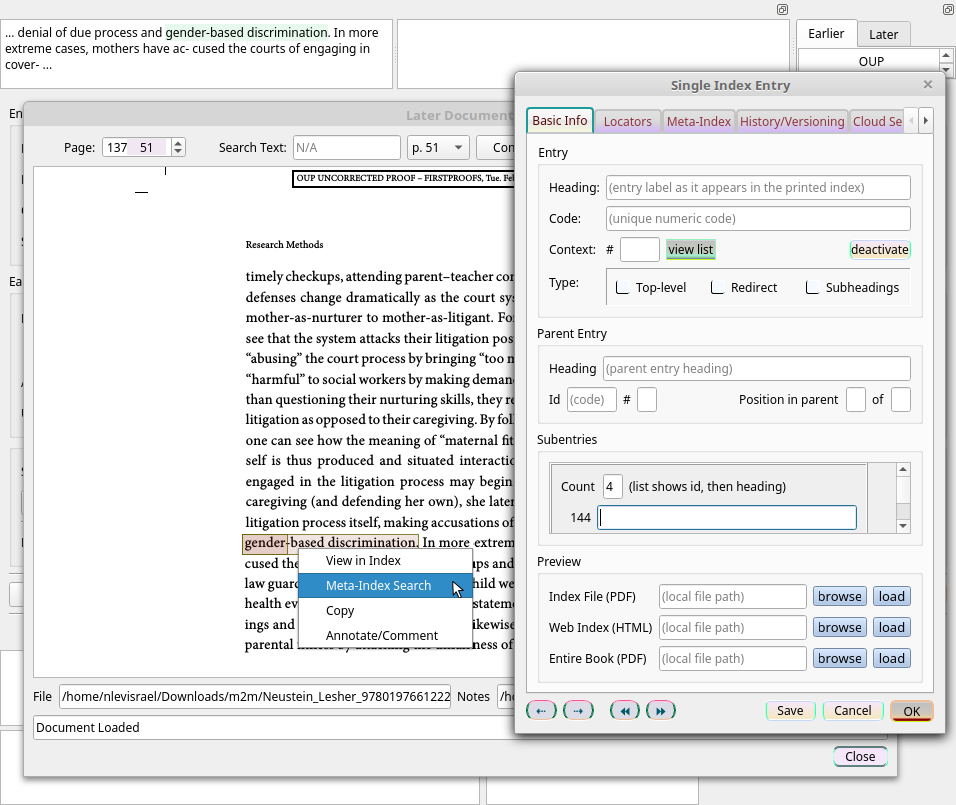
\includegraphics[scale=0.83]{fin/single.png}
\caption{An index entry dialog window (and context menu for single and meta-index views)}
\label{fig:ss1}
\end{figure}

\sstitle{Use Case 2: PDF Search for Creating and Updating Indexes}

\p{While curating an index, authors will often start by generating a basic list of terms 
relevant to the topic of the publication.  Given this list, they will 
then search for instances of those headings in the 
document text.  Although locators may often correspond to paragraphs without an exact match, 
a raw-text search can be a useful means to establish a provisional collection of locators 
that can be extended afterward.  A \PdfTk{}-enabled \PDF{} viewer lets users add 
words and phrases to a provisional heading-list --- or to the index index, once 
initially constructed --- by selecting a character-range in the \PDF{} document.  
Alternatively, a provisional list might be built from data files, plain text 
files, or from a different index (e.g., the prior edition of a 
book that is being republished).}


\begin{figure}[ht]
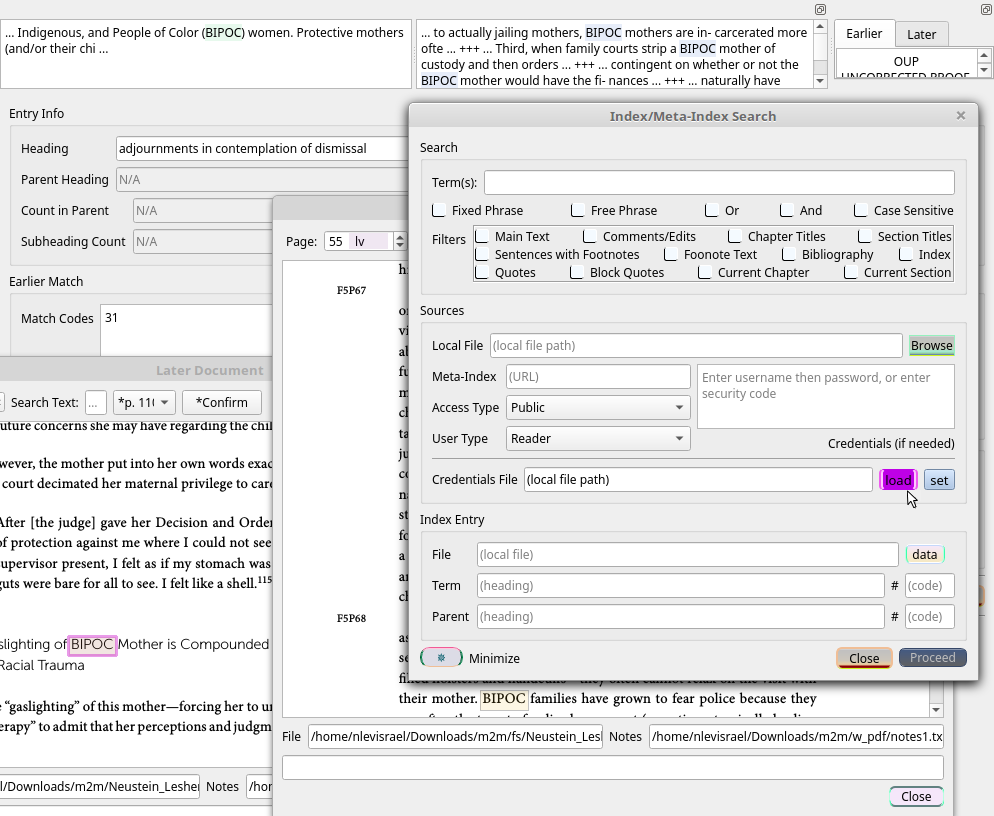
\includegraphics[scale=0.83]{fin/meta.png}
\caption{Dialog window for local and meta-index searches}
\label{fig:ss2}
\end{figure}

\p{When performing such initial matches, it is helpful to vary the order or precision of search terms.  
For example, a person's name in an index will typically be listed and alphabetized via last name first, 
but will usually be matched in the text in the opposite order, or last name alone 
(e.g., the entry \q{Durkheim, Emile} should be searched as \q{Emile Durkheim} or just \q{Durkheim}).  Likewise, 
instances of a single word within a phrase may be sufficient to confirm that the relevant stretch of 
text is indeed relevant for the entire phrase as a concept (for example, \q{House} in lieu of 
\q{House of Representatives}).  Given these points, \PacTk{} provides a front-end to 
\PDF{} search functionality which takes a provided search term (such as an index heading) and 
enables users to quickly rearrange or exclude words from the keyphrase to construct the 
specific match presented for \PDF{} search.  Successful matches are highlighted 
both in the \PDF{} page view and within secondary windows that show the raw text located 
within the relevant \PDF{} page (see Figure~\ref{fig:ss3}).  Presenting this contextual information allows 
the person compiling an index to verify that text matches are indeed conceptual hits for 
the relevant index entry, as opposed to false positives.}

\p{The screenshot in Figure~\ref{fig:ss3} actually 
represents a variation on index-building, where \PacTk{} was utilized 
to migrate an index for the second edition of a previously-published manuscript.  In this 
case, the first-edition index provided a provisional set of headings whose locators had 
to be updated with paragraph id codes for the new book.  We therefore employed a version of a
\PacTk{} \GUI{} that had two pairs of page and raw-text views.  In this variation, by 
matching terms against both documents, it is easy to confirm that a locator for the 
newer edition directly updates an index-entry from the prior book, by checking that the 
surrounding text is similar or identical.  Once entries are updated between the two versions, 
then new headings (plus new page/paragraph-id locators for old terms) can be added.}    

\begin{figure}[ht]
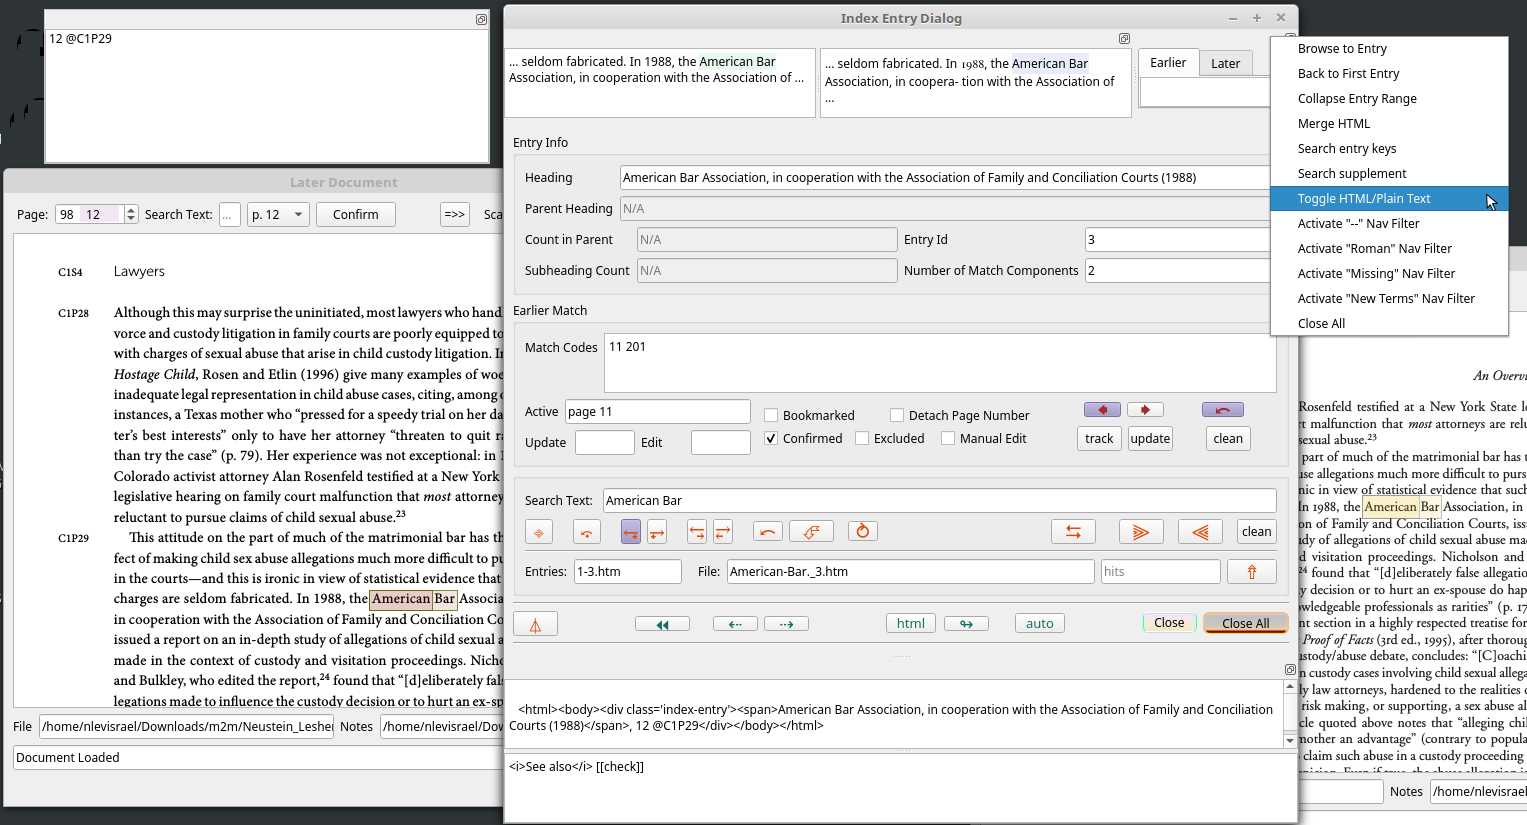
\includegraphics[scale=0.4]{fin/ie.png}
\caption{GUI functionality for compiling and curating indexes}
\label{fig:ss3}
\end{figure}


\sstitle{Use Case 3: Customizing GUI Tools for Indexing}
\p{The \GUI{}s in Figure~\ref{fig:ss3} include two distinct \PDF{} view windows, which might 
be used to review two different editions of a book whose index is being updated.  The software, that is, 
has two \PDF{} view windows to show the two editions, plus a central window with a variety of entry lines, buttons, and check boxes, intended to automate the data transfer (from old index to new) as much as possible.  After identifying all of the index terms from the prior edition and the corresponding page references, the software is designed to work through index entries one at a time --- either in alphabetized sequence or starting from a specific entry.  For each entry, users can click through the different page matches from the first edition, and the application then searches for similar terms in the second.  Above-mentioned search features enable users to fine-tune the search key to be more precise if needed --- for instance, inverting a proper name (Durkheim, Emile becoming Emile Durkheim), or restricting terms to the most important words (e.g., \q{`Diagnostic Impression' chart} might be reduced to \q{Diagnostic Impression}).  Making these adjustments by clicking buttons is quicker and easier for the user than typing new search terms manually.}

\p{Continuing the example of migrating from a first to a second edition, once search terms are matched against the new document, the code shows matches that are highlighted in both editions; and also shows the plain text of the corresponding files in separate windows.  It is worth mentioning that the highlights are constructed via native \GUI{} overlays, rather than employing the internal \PDF{} highlight mechanism --- the former is more flexible, and allows features like semi-transparency and color variation (which prove quite useful during a session where multiple entries and/or term-variants have been processed).  With these features, the user is able to quickly check whether a match replicates an entry in the first-edition index or else is a new paragraph-id locator.  In either case the user will click to register the match as appropriate for the new document's index and track the correlation between the old and new index --- the software automatically identifies correct paragraph-id codes if those codes, rather than page numbers, are used to generate an index.  When ready, the user can confirm that the data for the current heading is complete and proceed to the next one.  The software shown in Figure~\ref{fig:ss3} then generates \HTML{} code for that entry, which ultimately gets folded into the compiled second-edition index (this might be in formats such as Word, \PDF{}, \XML{}, etc.).  Users have the option of automatically storing the entry data on a web back-end, or via \FTP{}, which comes in handy if multiple people are working on an index at the same time.}

\p{Visible in Figure~\ref{fig:ss2} and Figure~\ref{fig:ss3} are numerous \GUI{} controls through which users can work through a list of entries via buttons, check boxes, context menus, and \q{dock} widgets (components that will either be affixed to the main window or float as separate windows, as desired).  Some of these controls help to quickly process individual entries; others affect the search process by filtering the target search area (e.g., restricting to certain pages --- such as a specific chapter --- or just to footnotes, etc.).  These various \GUI{} features enable the user to process a single entry much more quickly that manual text-editing.  Given a project for a second edition, for instance, often it is possible to confirm a match between the earlier and later document, and update the later index accordingly (with new locators), in just a few seconds.}

\p{When in the process of curating an index, it may be important to examine \PDF{} representations 
in several different variations.  In particular, looking directly at document content as internally 
represented can clarify anomalies such as false negatives (caused by hyphenation, ligatures, 
nonstandard fonts, etc.).  In other cases, raw text might provide more convenient visualization 
for the text around a match than is evident in the fully-rendered \PDF{} view.  The 
components show in Figure~\ref{fig:ss3} present document content in three contexts: the \PDF{} view itself; 
the unadulterated raw text for a given page; and an edited version of the raw text simplified 
so as to emphasize context around a match (in each case the match itself, if present, is 
highlighted with an overlay).  The simplified raw-text view presents a window of approximately 
30 characters on either side of the matched characters (users can reconfigure the exact number) 
allowing users to quickly check which words appear to the left and right of a given 
match.  Such functionality helps one to double-check that a raw match is conceptually 
appropriate, or to determine the proper subentry within which to include the current locator 
(\q{gender bias}, for example, could be divided into gender bias \textit{in courts}, 
\textit{in hiring}, etc. --- glancing at whichever words surround the matched \q{gender bias} 
string might facilitate the user deciding which subheading is most appropriate). 

}


\p{Whether building an index from scratch or updating an earlier publication, these \GUI{} capabilities streamline the indexing process.  Rather than typing index entries directly into an index file --- manually adjusting details like italics, subentry lists, roman vs. arabic numerals, and so forth --- the user could rely on mouse clicks and context menus (with minimal actual typing) to compile a data structure holding all of the index entries.  A human-readable index is then generated from that structured data, or authors could submit the index as a data file instead, which could be incorporated into Meta-Indexes discussed below.}

\p{The \PacTk{} \GUI{} tools are designed to flexibly interoperate, with few external code dependencies and an emphasis on autonomous, modular design.  That is, individual window components and/or algorithm libraries may be 
combined together and fine-tuned for specific book projects.  In the example discussed here, our 
requirements involved migrating data from an older edition of a book to a new index.  
Other publications might have different needs --- 
for example, syncing an index to a published data set; or compiling an aggregate index from a volume with individual chapter authors.  Modular, native-compiled \GUI{} controls permit new secondary windows to be implemented so as 
to support convenient user interaction, or automation, to complete tasks requisite for specific publication's 
workflow (see the summary of \BdQS{} below for more info on dynamic \GUI{} customization).}

\p{A display with two \PDF{} views may also be helpful for working on a single document.  One window can 
show the text which an author or editor is currently addressing, while a second window could show 
content from a different chapter or section of the same book/article.  This would operationalize side-by-side 
comparison, such as to check that earlier language is not repeated, or to ensure that a particular 
bibliographic reference is cited in at least one paragraph where the concomitant 
publication (or its topic) is discussed.}




\vspace*{12pt}
%{\semihr{0.377\textwidth}}
{\semihr{0.437\textwidth}}
\vspace*{5pt}
%\sectnum{1.}
\hspace{2pt}\secttitle{{II \hspace{2em} Meta-Indexing, Cloud Services, and Text Mining}}
\vspace*{5pt}
{\semihr{0.437\textwidth}}

\vspace*{3pt}


\sstitle{Use Case 4: Annotated PDFs as SVG Files}

\p{\lPDF{} annotation capabilities (which include editing features and comment boxes) are unfortunately very limited.  
Many \PDF{} viewers cannot show annotations at all; those that do, often present annotations in small, 
hard-to-read box areas.  Annotation support is not uniform: 
when a file is shared, there is no guarantees that recipients will be able 
to see annotations at all, or that they are presented in a usable manner.  One solution to this 
problem is to convert \PDF{} documents to a series of 
\SVG{} files, that can be browsed as individual pages.  \lSVG{} is a general-purpose format for 
creating \TwoD{} graphics, and \SVG{} versions of \PDF{} pages can be annotated with overlays that 
employ the full range of \SVG{} capabilities, including all mathematically-describable paths and shapes; 
semi-transparent colors; scalable text; and mouse/keyboard user interactions.  
For example, some actions performed in the process of editing page proofs may be 
more user-friendly (in terms of \GUI{} interactions and User Experience) when the 
document is read through an \SVG{} viewer rather than a \PDF{} viewer.}

\p{Figure~\ref{fig:ss4} shows a feature wherein annotated \PDF{}s are converted to \SVG{} files so as to better visualize the annotations (which in ordinary \PDF{} viewers tend to be reduced to poorly-formatted comment boxes).  Here the comment-text 
is enlarged and color overlays clearly identify which sections of text correspond to specific 
annotations.  Figure~\ref{fig:ss5} reflects special programming for a project where annotations were 
grouped into different categories, modeling linguistic/discursive properties of the \PDF{}-rendered content; 
a master index was then compiled associating specific pages to the annotation categories, with hyperref 
links to access the individual pages as desired.}

\begin{figure}[ht]
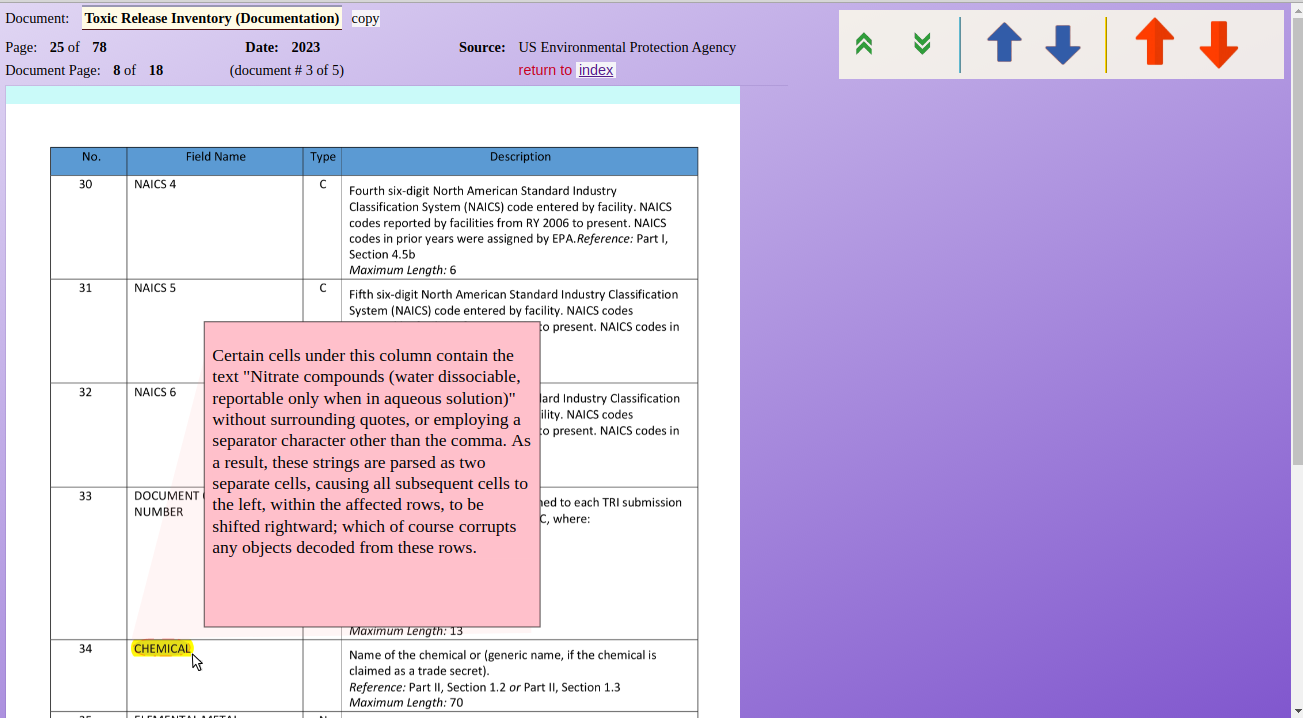
\includegraphics[scale=0.8]{fin/tox.png}
\caption{Mapping PDF pages to SVG views for improved annotation support}
\label{fig:ss4}
\end{figure}

\p{One benefit of \PDF{}-to-\SVG{} conversion is that \SVG{} files thereby become independent resources that 
can be individually hosted online.  Most web browsers have \PDF{} plugins, so that \PDF{} files can be 
viewed without being downloaded, but there are no guarantees that users will also be able 
to see \PDF{} annotations in the browser.  Moreover, there is no way to construct a hyperref 
link to a single page, section, or chapter; only to the \PDF{} as a whole.  With \SVG{} files, 
on the other hand, each page will potentially have its own web \URL{}, and links to single pages may be 
embedded in web resources (and also other \PDF{} documents).  Such web links can be useful for collaborative 
editing as well as referencing pages in files already published.}



\begin{figure}[ht]
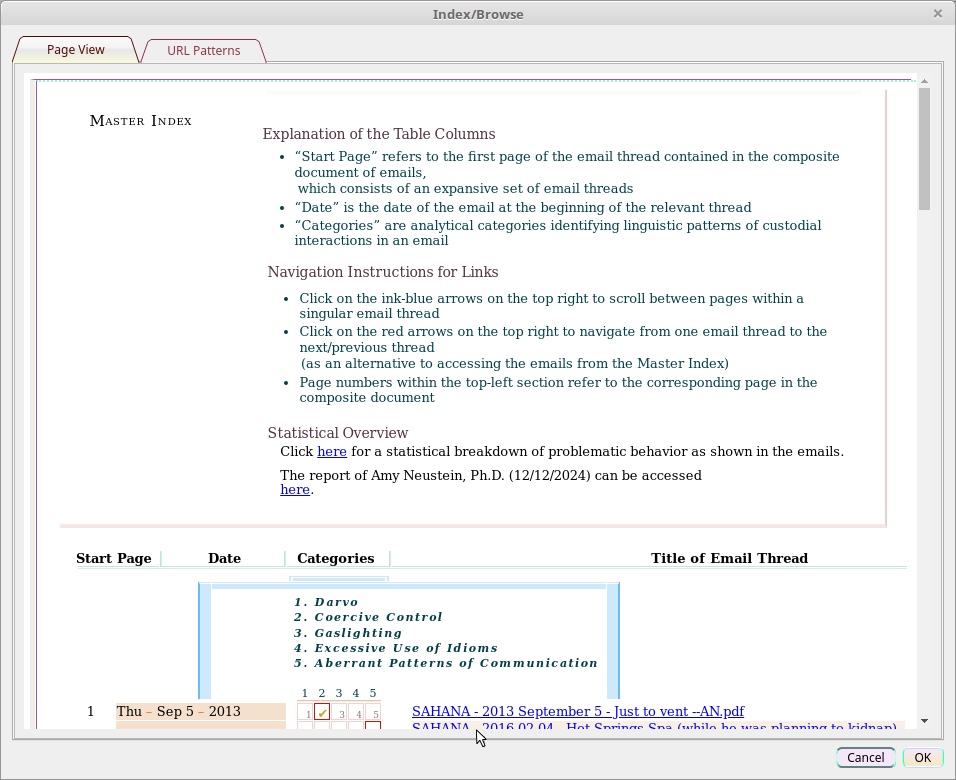
\includegraphics[scale=0.5]{fin/sah.png}
\caption{A category-based web-accessible index table for SVG pages}
\label{fig:ss5}
\end{figure}

\begin{figure}[t!]

\includegraphics[scale=0.5]{fin/stark-mi.png}
\includegraphics[scale=0.5]{fin/stark.png}
\caption{Meta-Index Search through a Web Portal}
\label{fig:ss6}
\end{figure}



%\vspace*{-1em}

\p{\lPacTk{} additionally supports technology for embedding web viewers in standalone native 
(i.e., desktop-style, rather than web-based) applications.  In this manner, 
authors/editors can preview the appearance 
and functionality of \SVG{} annotations before they are disseminated online.  Special-purpose 
native/JavaScript interop allows the host application to respond to a wider range of 
user actions than browser-based code in isolation, so \PacTk{} tools can be used to 
modify and style annotations, edits, and comment boxes while working directly with \SVG{} files. 
By default, \PacTk{} implements web/native interop via \textbf{QWebChannel}, one 
technology within the \Qt{} application-development libraries.  The combination 
of \textbf{QWebChannel}, \PDF{}, and \SVG{} is a powerful but rarely used 
programming paradigm.  In addition to document publishing, browser-embedding can be a 
convenient tool for curating data sets, particularly in contexts such as 
\GIS{} that often rely on a web interface for data acquisition; and for programming 
dataset-backed simulations (especially when user input/gestures are involved).}



\sstitle{Use Case 5: Curating Meta-Indexes}

\p{The benefits of indexes for enhancing local text search may certainly be extended to 
more general web/database searches.}


\p{Because \PacTk{} represents indexes via metadata, it is straightforward to merge 
indexes from multiple documents into an aggregate database, also known as a 
\q{meta-index.}  Meta-indexes 
may be compiled for individual book series; academic journals; or even large-scale 
document corpora.  Such meta-indexes could be made available to users in one of two 
ways.  On the one hand, users might enter search terms and query against an encompassing 
bibliographic database, without necessarily starting from one specific book 
or publication.  Alternatively, a user might be reading a specific digital 
publication and request a local search that then expands to include a meta-index.  
That is, users could indicate an interest in match-results not only for the book 
they are currently reading but also for pages in other volumes stored alongside it 
in a book series or corpus archive.}



\p{Hosting and curating a meta-index is facilitated by \PacTk{}'s structured 
metadata format.  Because all books in a series/archive will share a metadata profile, 
new indexes can be merged into a preexisting database as soon as they are finalized.  
\lPacTk{} provides an \API{} protocol for registering a new index as well as 
querying for results in a hosted meta-index.  \lPacTk{} also offers native \API{} tools 
such that \PDF{} viewers can query against a database when expanding local  
to meta-index searches.  Meta-index \API{}s could likewise be used for search front-ends 
exposed to users via web pages for specific journals, book series, abstracts aggregators, 
and analogous publishers' web content.}

\p{Via conventional \q{forward indexing,} new documents become merged into composite 
search \q{indexes} as soon as they are published.  The term \q{index} in this content 
refers to word-by-word counts on the principle that the number of occurrences of some 
word or phrase, in a given document, provides a rough measure of the document's 
relevance to that word.  More refined algorithms can modulate relevance scores 
by considering conceptual associations, and, in general, the phenomenon 
of multiple expressions designating the same (or closely related) referents 
(e.g., \q{the President} and \q{the White House}).  Actual book indexes, of course, 
represent a more detailed model of such conceptual relationships because 
authors/editors explicitly select a set of terms that are especially 
significant for the material's theme/topic; and also consciously choose 
which conceptual links to explicate (via \q{see also} clauses, in particular).  
Meta-indexes can, of course, be layered on top of automatically-indexed 
search engines.}

\p{Whether or not meta-indexes work against a data set that includes a 
full search-engine database, the information content of a typical meta-index 
will be sufficiently large that query processing functionality would have 
to be hosted on a publicly-accessible server.  In many use-cases, a web- or 
cloud-based meta-index would be accessed from a single \PDF{} file --- 
we assume the reader initiates a meta-index search on the basis of 
material they are reading in the local file --- in which case 
remote queries, through an \API{}, could be sent and received 
by a conformant \PDF{} viewer.  In such contexts, users would 
not see the web/cloud content directly.  However, publishers 
have good reason to also wrap meta-index access in a 
modern-style web site, for the alternative use-case 
wherein a researcher does not start from a particular 
book but rather visits a web portal to find materials 
on a topic that interests them.  Figure~\ref{fig:ss6} 
shows a hypothetical web front-end along with a 
screenshot with an example of two books from the 
same series, that could be linked by behind-the-scenes 
searches.}


\p{Existing bibliographic aggregators, such as Dimensions, pair \API{} protocols with 
customized query languages for bibliographic databases.  To support such technology, 
\PacTk{} includes code for a Bibliographic-database Query Infrastructure  
(\BdQS{}) for exchanging structured data with \API{} hosts.  Instead of 
\REST{}-encoded \URL{}s, more complex query prompts (and responses) can be encoded 
via \BdQS{} for \POST{} requests (native-compiled code can leverage easy-to-use 
request builder objects).  The \BdQS{} framework actually has several 
use cases within \PacTk{} alongside \API{} query factories; other use cases 
related to \GUI{} programming were mentioned earlier.}

\p{The \PacTk{} code base additionally includes prototype Cloud-Native service implementations 
for hosting meta-index databases.  These cloud applications --- which are able to be 
developed and tested as self-contained desktop components before getting 
deployed online --- encapsulate many details of meta-index management, database 
admin, and \API{} support, with significant code reuse between native/desktop 
clients and \API{}/cloud server endpoints.}


\begin{figure}[ht]
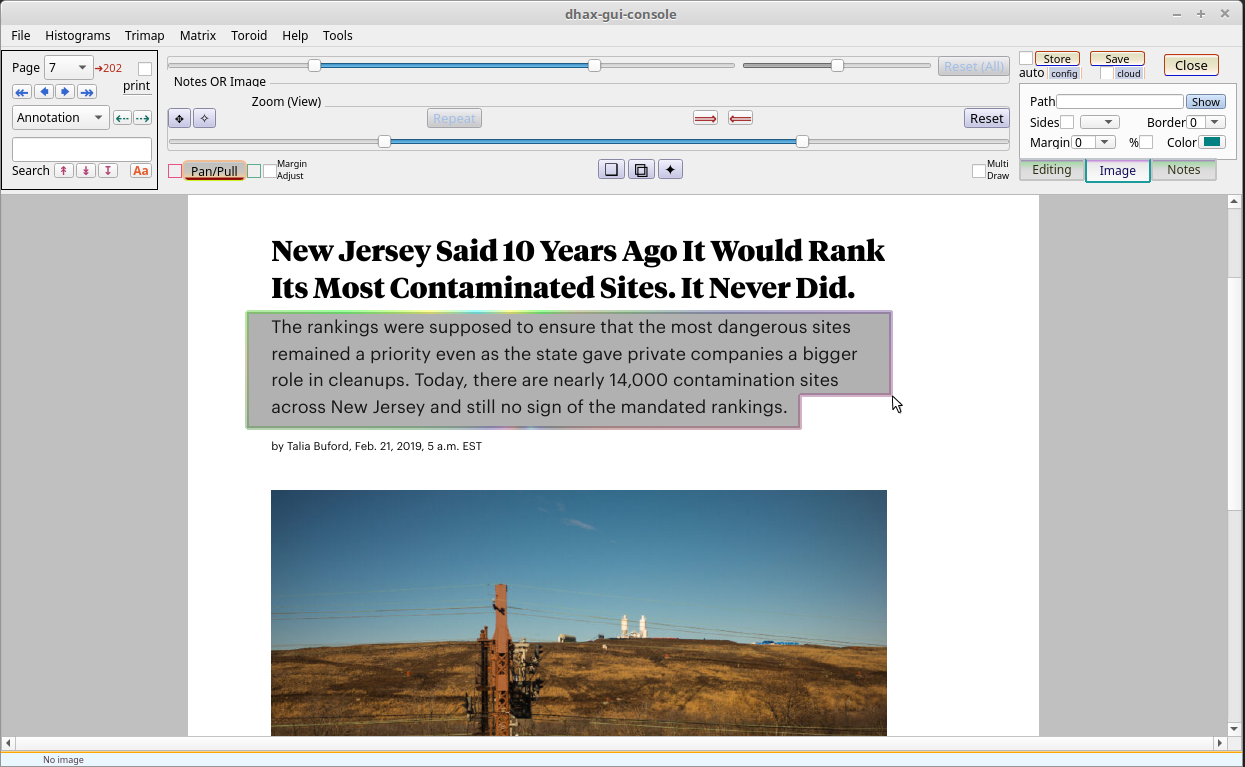
\includegraphics[scale=0.5]{fin/oct.png}
\caption{Flexible range-select features}
\label{fig:ss7}
\end{figure}

%\vspace*{.5em}

\sstitle{Use Case 6: Machine-Readable Text Encoding}

\p{Because launching \PDF{} text search for each \API{} query would be very inefficient, 
cloud-based meta-indexes must compile machine-readable representations of 
text document contents, so as to search many books at once.   This process also corrects for the 
inherent limitations of \PDF{} text searches, which can be counter-productively 
stymied by such basic typographic conventions as ligatures, end-of-line hyphenation, 
apostrophes, footnote marks, and many other familiar presentational details.}

\p{With full metadata in place, \PacTk{} indexes construct in-document locators that 
combine two different target origins.  On the one hand, text spans are declared 
via machine-readable encoding for text mining, rather than (or in addition to) 
the internal \PDF{} text representation, which is often an incomplete representation 
of the document text as understood by human authors and readers.  Concordantly, 
on the other hand, 
the visible outlines of text-segments that match index terms are stored 
via \PDF{} page coordinates, which may be traced by \SVG{} or other graphics overlays.  
In both cases, the internal \PDF{} searching and highlighting functionality is 
supplanted by a two-facet text and graphics representation.  Ordinary \PDF{} 
search may be employed initially to \q{bootstrap} an index, but once finalized 
the document metadata would be consulted as a basis for searches both locally 
and via \API{}s.} %\newpage{}

%\vspace*{-1em}
\p{Rigorous text encoding can also improve User Experience working locally 
with \PDF{} files.  For example, users could copy the text of a full 
sentence where a match occurs --- not just the search term itself --- with a single 
button-click.  Figure~\ref{fig:ss7} shows a range-select option that syncs mouse drags with key-presses to select a multi-line area that extends to the margins in the middle lines (a useful alternative to ordinary \PDF{} ranges that can only be a simple rectangular box, thereby either cutting important words from left or right or including extraneous words around the range's start and end, which makes it difficult to 
select a full sentence or other meaningful unit of text).  
Advanced \GUI{} programming in conjunction with machine-readable 
text encoding permits users to accomplish their goals in find, copy, and remote-search 
functionality with less hassle than traditional \PDF{} viewers 
(which rely on flawed internal text representation).}

\begin{figure}[ht]
\includegraphics[scale=0.45]{fin/ling.png}
\caption{Enhanced GUI capabilities enabled by machine-readable text encoding}
\label{fig:ss8}
\end{figure}


\vspace*{6pt}
\sstitle{Use Case 7: Rigorous Text Mining}
\vspace*{3pt}

\p{The limitations of \PDF{} text encoding serve as a hindrance to advanced text-mining 
algorithms.  These lacunae became evident during the Covid pandemic, when scientists sought to 
gather intelligence from a broad pre-pandemic literature about Coronaviruses and the first 
(2002-2004) \SARS{} outbreak, as well as new publications which quickly emerged summarizing 
research into \SARSCoV{}.  The Allen Institute for \AI{} (\AItwo{}), for example, compiled a 
large \CORD{} corpus using a project-specific \JSON{} encoding of all document 
texts.  However, \AItwo{} pointed out that transcription errors were limiting the 
effectiveness of text-mining algorithms implemented against the corpus 
(an extended analysis of \CORD{} and other Covid-related data integration 
projects can be found in our book \textit{Innovative Data Integration and Conceptual Space Modeling 
for COVID, Cancer, and Cardiac Care}, Elsevier, 2022).  We identified problems such as inconsistent representation of medical and chemical terms/formulas --- such that correlations between publications 
were not properly identified --- and ambiguities in modeling the structural 
breakdown of natural-language text into paragraphs and sentences.  \lAItwo{} argued that new 
machine-readable text formats were necessary, rather than relying on \PDF{} representations, 
and issued a \q{call for action} encouraging publishers and scientists to develop 
modernized text-encoding and metadata standards.  We thereby developed a novel 
document-preparation system that generates structured text representations alongside 
conventional \PDF{} files, which we used for composing the data-integration book mentioned 
above (and subsequent publications).}

\p{\lPacTk{}-enabled documents can utilize similar representations to expose full text content, 
alongside index metadata, to bibliographic databases.  Rigorous encoding permits 
databases to systematically address ambiguities related to match contexts and query 
results.  Suppose an \API{} request models a search for a keyphrase and 
requests all sentences where the phrase appears, among a multi-document collection.  
In order to fulfill the request, a query engine would need to clarify the proper 
representation of a \q{sentence,} as well as adjust for anomalies such as intra-word 
hyphenation.  For example, requests for complete sentences may or may not 
specify that the content of footnotes or block quotes inside the sentence 
should be included.  Or, the preliminary language preceding an enumerated or 
bulleted list might be considered a single sentence (even if it ends with a 
colon rather than a period), but in some contexts that preamble together 
with the overall list serve as an aggregate sentence.  Apart from intra-document 
queries, such granular discursive constructs can be addressed by plugins to 
search-engine tools that could be employed as meta-index back-ends 
(see Figure~\ref{fig:ss9}).
}

\p{In short, rhetorical features such as footnotes, quotes, figure illustrations, 
enumerations, and itemized lists all represent discursive structures that complicate the 
straightforward breakdown of text into sequences of paragraphs and sentences.  Enhanced 
search, in particular, should allow queries to filter search targets into 
footnote text, section headings, chapter titles, quotes (inline and/or block), 
content within figures/diagrams, and annotations/comments, as well 
as document text in general.  Query protocols 
should therefore recognize a plurality of discursive structures both to 
establish search parameters and to clarify the desired scope for contextual 
data (the screenshot in Figure~\ref{fig:ss8} presents a visual example).  
These details can be exposed to \API{}s via \PacTk{}'s \BdQS{} framework.}

\begin{figure}[h!]
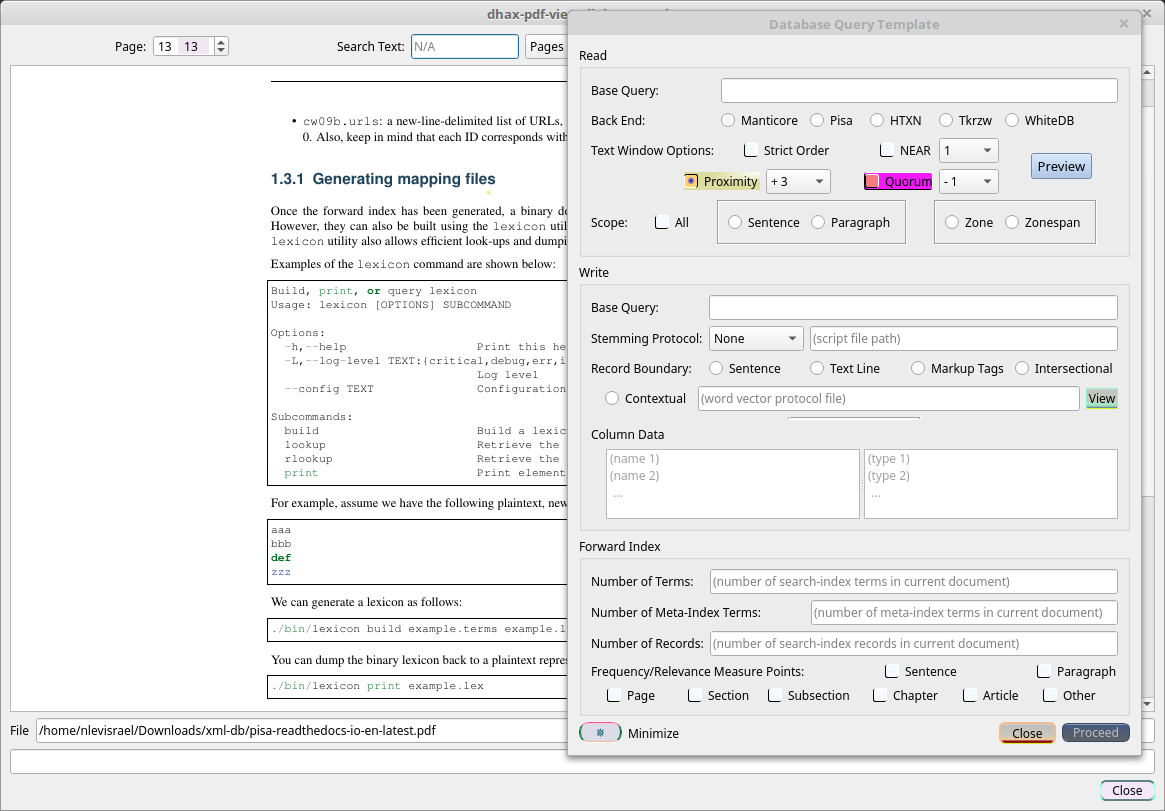
\includegraphics[scale=0.66, trim=8.4cm 0 0 0, clip]{fin/pisa.png}
\caption{Configuring Default Back-End Queries}
\label{fig:ss9}
\end{figure}




\vspace*{20pt}


%{\semihr{0.13\textwidth}}
{\semihr{0.197\textwidth}}
\vspace*{5pt}
%\sectnum{1.}
\hspace{2pt}\secttitle{{III \hspace{2em} Data Publishing}}
\vspace*{5pt}
{\semihr{0.197\textwidth}}

\vspace*{11pt}

\sstitle{Use Case 8: Deserializing Data Files}


\p{In contemporary publishing, text documents are often paired with 
scientific data sets in accord with \FAIR{}sharing research-transparency 
principles (\q{\FAIR{}} stands for Findable, Accessible, Interoperable, Reusable).  
For someone intending to examine published data sets, raw data files are 
of limited value.  Sometimes data sets can be loaded into proprietary 
software used by research labs, but many readers will not necessarily 
have access to such software (thereby failing the Accessibility and Reusability 
criteria).  Consequently, individual scientific disciplines are often 
associated with domain-specific data publishing formats that are paired with 
dedicated deserialization tools (i.e., computer code which 
reads raw data files into live memory, without relying on special-purpose 
software).  Such code libraries are often maintained by individual 
institutions or organizations, such as academic departments, on behalf of a 
broad research community.  Examples include \FASTQ{} and \VCF{} for genomics; 
\FITS{} and \netCDF{} in astronomy and earth sciences; \PDB{} and \MOL{} in biochemistry; 
\IFC{} in engineering; \SEGY{} and \BAG{} 
for geophysics and oceanography; \CoNLLU{} in computational linguistics; 
\DICOM{} and \OMETIFF{} for bioimaging; and \GIS{}-indexed attribute layers 
and shapefiles for geospatial data sets.  Among many others: this list is not at all exhaustive.}


\p{Some domain-specific file formats are derived from general-purpose formats 
such as \CSV{}, \XML{}, and \JSON{}.  Others use idiosyncratic text and/or binary 
serialization protocols, so that custom parsers are necessary so as to consume byte or character 
streams from raw data files.  Even when the actual encoding is performed via a 
generic standard like \XML{}, dedicated deserialization code will still be needed --- 
generic parsers can convert a given \XML{} document to a Document Object Model 
(\DOM{}) infoset, but algorithms will have to navigate the document hierarchy and extract 
text strings from element nodes, which become the input for initializing 
object data fields.}

\p{In principle, supplying code libraries for parsing raw text files and/or 
traversing infosets embodies \FAIR{} standards by ensuring that a typical 
reader who accesses published books or articles can likewise obtain usable 
research data.  In practice, however, code libraries can lag behind 
the evolution of data standards, and \FAIR{} access may be hindered by 
programming/technological minutiae: versioning conflicts, programming language barriers, operating-system 
conflicts, and similar obstacles.  It is difficult to consistently maintain 
code libraries for a variety of different operating systems, coding languages, 
computational environments, and non-backwards-compatible versions of 
external dependencies, especially when the data format targeted by a library 
itself goes through multiple changes.}
   

\p{\lPacTk{} seeks to address these concerns by engineering the \BdQS{} framework 
to support data deserialization as well as bibliographic database queries.  That is, 
deserialization algorithms can be expressed in \BdQS{} and compiled to a 
custom Intermediate Representation/bytecode stack. \lBdQS{} is implemented in 
largely self-contained native code than can be dropped as source files into 
any \Cpp{} project (or compiled into dynamic libraries invoked by scripting 
languages).  As a result, \BdQS{} can be ported to many diverse environments 
and embedded into many scientific applications, thereby ensuring that up-to-date 
deserialization capabilities are accessible for any file type for which 
a \BdQS{}-based parser has been published.  The entire \BdQS{} stack could moreover 
be released as part of the source code contained in a published data set, 
so that deserialization functionality becomes part of the data set's overall package.}

\p{In general, \BdQS{} deserializers can either parse character-streams 
directly --- by registering callback functions responding to matches in 
Regular-Expression-like pattern language --- or else post-process 
\XML{}, \JSON{}, \CSV{}, and similar formats by declaring handlers for traversal 
events.  \lBdQS{} provides a flexible suite of overload and redirection 
protocols to marshal post-parse navigation algorithms to \Cpp{} methods 
that can granularly model preconditions for reading specific data fields 
(e.g., required nonempty, numeric range-validation, controlled vocabularies 
for string columns, etc.).}



\sstitle{Use Case 9: Data-Set Visualization and Nanopublications}

\p{Embedding deserialization code is a good illustration of \FAIR{}sharing priorities: 
ideally, all the resources necessary to (re)use a data set should be provided as 
part of the data package itself, rather than expecting users to download 
separate dependencies from external sources.  Similar goals inform the 
design of data visualization features specific to individual data sets.}

\p{Some data sets might be loaded into readily-available software, but in many 
cases code for visualizing and studying raw data files should be provided 
as part of the data set itself.  In these situations, the package 
can include source code files that, once compiled, produce an 
executable program which renders the concomitant data set in a 
visual, interactive manner.  This may involve the use of charts or 
plots to show statistical trends; as well as structured \GUI{} controls, 
or separate windows, to display the attributes of individual data objects.  For the 
purpose of discussion, we refer to such self-contained resources specific to 
an individual data set as \q{Data Set Applications} (\DSA{}s).}

\p{When a document (book or article) is explicitly paired with a 
published data set, information about the data set should be 
included in index/search metadata.  This would allow 
keyword searches to be extended to raw data fields, as well 
as data-structure parameters (such as column labels, source-code 
annotations, procedure names, etc.).  Moreover, sections of text 
can be isolated as cross-references for data-structure parameters 
as well as individual objects/records.  For example, a specific 
column or field in tabular data structures can be cross-referenced 
with the paragraph in article text where that field is 
discussed (its observation/acquisition methodology, units of measurement, 
statistical distribution, etc.).}

\p{\PacTk{}, in particular, envisions \PDF{} documents links to supplemental 
resources that could take the form of graphics displays (showing 
things like statistical summaries) or dedicated \GUI{} windows (showing, 
for example, structured data in tabular or hierarchical fashion).  
This model of supplemental presentations comports with the 
emerging idea of \q{nanopublications,} which are independently 
citable works that are typically smaller in scale than, but 
may be paired with, a research article.  Depending on one's preferred 
definition, an interactive statistical diagram, or a \GUI{} window that can browse 
through discrete objects/records in a data set, may be considered a nanopublication 
or an integrated collection of multiple nanopublications.  In either case, 
\PacTk{} allows the nanopublictions associated with a research document to be 
accessed interoperably from \PDF{} (or \SVG{}) files via the same conventions 
as indexing and text searches; and allows nanopublications to be 
integrated with meta-index databases for holistic corpora.} 
 

\sstitle{Use Case 10: Microcitations and Multimedia Cross-Referencing}

\p{Cross-referencing between research papers and data-set nanopublications 
is a special case of multi-media cross-referencing, where annotations defined 
in the context of a specific media type assert semantic or thematic 
relations to content with a different modality.  Concrete examples 
of multimedia cross-referencing include geotagging video frames; linking 
\CAD{} digital twins with product specs; annotating Regions of Interest 
within image series with coded labels associated with published raw data; 
embedding tags in 360\textdegree{} displays whose content includes 
\URL{} strings that encode identifiers for data set objects; developing 
color- and/or shape-coded attribute layers for \GIS{} overlays (so users 
can browse between digital maps and structured object 
displays); and constructing numeric tuples from \ThreeD{} graphics scenes 
such that particular camera orientation/location and zoom levels 
can be recorded as a unit, allowing the relevant \ThreeD{} content to be 
repeatedly visualized from a specific perspective (in other words, 
links can be embedded in \PDF{} files, web pages, software, or any 
other context so that users can reconstruct a specific \ThreeD{} state, 
as constituted by camera angle/location and zoom settings).}

\p{The challenge when implementing multimedia cross-references is to 
ensure that viewers for two divergent media types can properly 
interoperate.  With correctly interpreted cross-references, application users should be able 
to navigate from a window dedicated to one media/file to a 
window rendering a different format, and correctly isolate the 
portion of a file (not just the overall file) implicate in a cross-reference.  
For example, geotagging video frames should enable users to pause a video 
at a particular location and then, via the geotag, switch to a map 
display centered on the geospatial coordinates visible in the video 
(consider, e.g., a video documenting progress in an environmental 
remediation site).  Conversely, \GIS{} attribute layers would represent 
locations for which video content is available, and allow the users 
to watch the relevant videos starting from the appropriate time-point.  
Such interoperability is only possible if the components and/or applications 
responsible for rendering the two content-types share a common 
annotation and message-passing protocol.}


\p{The \PacTk{} code base includes prototype viewers for some 
widely-used media types, including video (and audio) players, 
digital maps, 360\textdegree{}/panoramic photography, \ThreeD{} 
triangular-mesh displays, image series, and parse-representation 
formats associated with text mining and computational linguistics.  
These prototypes illustrate how cross-referencing protocols 
may be adopted, and can be extended to provide domain-specific 
plugins for \PDF{} viewers or bundled into data-set application code.  
More generally, \PacTk{} defines a cross-referencing protocol that 
ensures proper interoperability between multimedia displays 
and text/bibliographic databases.  This protocol can then 
be adapted for other media types, including special-purpose 
formats specific to individual scientific disciplines 
(such as \ThreeD{} displays for molecular visualization, in cheminformatics; 
Digital Model Repositories for oncology and other biomedical 
fields; radiomic biomarkers for diagnostic imaging; 
and audio files with waveform visualizers for spoken-language corpora).}

\p{Standardized cross-referencing protocols enable scientific 
applications to interoperate with assets from the full range of media types that 
might be published (as supplemental 
materials) alongside research works.  Rather than relying on generic \PDF{} viewers, scientists 
could then employ \PDF{} applications specifically 
engineered to work with the data formats and visualization 
strategies specific to a given research discipline.  Comments  
and annotations within data-set source code can serve to document 
the data set as a whole, but --- aside from semi-formal code 
annotations  --- similar (and potentially more rigorous) details may 
be intrinsically expressed in code via declarations recognized 
by and incorporated into the compiler pipeline, and exposed 
through runtime reflection and queryable intermediate representations.  
\lBdQS{} in particular, more than conventional languages, 
encourages systematic introspection for \GUI{} objects and 
their interrelationships, such that correlations between 
data-set entities and their user-interface representations 
may be rigorously identified.}


\vspace*{8pt}

%{\semihr{0.513\textwidth}}
{\semihr{0.5785\textwidth}}
\vspace*{6pt}
%\sectnum{1.}
\hspace{2pt}\secttitle{{IV \hspace{2em} Documenting Data Profiles via Code Annotations and Conventions}}
\vspace*{4pt}
{\semihr{0.5785\textwidth}}
\vspace*{7pt}

\p{Publishing code alongside raw data sets facilitates accessibility and reusability.  
In addition, properly engineered computer code can augment data sets' 
explanatory and pedagogical dimension.  Any information aggregate 
represents specific data \q{profiles} and acquisition modalities.  
Often these are informally discussed in research papers, but data sets 
themselves can document their observation protocols, pre-analytic 
transformations, statistical properties, and theoretical assumptions 
through annotations, type interfaces, and coding conventions.}

\p{In particular, \q{design by contract} programming techniques become 
particularly valuable in scientific-computing contexts.  These techniques 
explicate what are otherwise merely implicit technical and theoretical 
assumptions.  Preconditions on procedures, object attributes, and 
data-type constructions can specify units of measurement, 
valid ranges for numeric values, collections-type constraints 
(e.g., that two lists have the same number of elements), algorithm 
prerequisites, and similar expectations presupposed by the 
implementation of one or more function-bodies.  The overall 
collection of contracts declared for a class interface 
or code library serves to illustrate theoretical 
paradigms germane to research from which data sets are 
compiled. Manifesting such contracts in computer code, 
not just as abstract or mathematical conventions, 
concretizes theoretical constraints in an environment 
that lends itself to exploration and visualization.}

\p{Analogously, algorithms expressed in computer code 
are amenable to being studied interactively, more so that quantitative 
formulae.  By varying algorithms' sample domain, parameters, and scope 
--- plus examining intermediate results --- researchers 
can get an experiential grasp on quantitative constructions
that might be harder to understand when presented just as 
cryptic equations.}

\p{Similar clarification can derive from a type system.  There are many 
variations on a basic number-pair, for instance, differing in terms of 
how coordinates are labeled (x/y, row/column, width/height, etc.).  Mixing 
incompatible pairs (vertical then horizontal and vice-versa, say) is a 
common source of coding errors, which may be avoided by construing 
each coordinate system as its own type (so a width/height pair could not 
be added to a row/column, for example).  These type-level coordinate constraints 
document data-modeling paradigms for analogous reasons.  A related 
example would be specific types for representing constrained character arrays, 
that are less flexible than generic strings but imperfectly 
encoded by straightforward numeric types (a good example is 5- or 9-digit US zip codes, 
which are not ordinary numbers because they need a specific digit count, and because 
leading zeros are significant).  Within \BdQS{}, 
granular number-pair (and number-tuple) types as well as \q{constrained 
character arrays}) are built-ins with special syntactic and introspection support.}

\p{Given these considerations, \PacTk{} engineers the \BdQS{} 
environment to prioritize this pedagogical and 
replication-oriented dimension.  \BdQS{} spans a compiler 
and runtime infrastructure that highlights computational 
details which are intrinsic to data sets' scientific 
provenance, such as multiple-dispatch in terms of 
contract satisfiability and type-level guards for 
measurement scales and dimensional analysis.  Accordingly, in addition to 
employing \BdQS{} for bibliographic queries and deserialization, 
data-publishing curators may benefit from a \BdQS{} scripting 
environment for analytic and \GUI{}-integration tasks.}

\vspace*{11pt}

{\semihr{0.097\textwidth}}
\vspace*{4pt}
%\sectnum{1.}
\hspace{2pt}\secttitle{{Video Links}}
\vspace*{4pt}
{\semihr{0.097\textwidth}}

\vspace*{4pt}

\p{For more information, please see our software demo videos, which show 
software components that could be integrated into dataset applications 
and \PDF{} viewers:

%\vspace*{14pt}

% \href{http://www.lingtechsys.com/videos/qmt-composite.mkv}{\parbox{.3\textwidth}{\includegraphics[scale=.3]{pm/qmt-composite.png}\\\GIS{}}}%
% \hspace{10pt}\href{http://www.lingtechsys.com/videos/dhax-composite.mkv}{\parbox{.3\textwidth}{\includegraphics[scale=.255]{pm/dhax-composite.png}\\360\textdegree{} photography}}%
% \hspace{25pt}\href{http://www.lingtechsys.com/videos/xcsd-composite.mkv}{\parbox{.3\textwidth}{\includegraphics[scale=.35]{pm/xcsd-composite.png}\\Image Processing}}%

}





\vspace*{3pt}

\pagestyle{lastpage}
%


%\p{}


\end{document}

% Figure 1  ZoLa compared with a static \\PDF{}{} map
% Figure 2  Merging NYC environment-related classifications 
 %            with WRI and ISI designations
% Figure 3  Custom query windows for accessing E-Designation data
% Figure 4  Customizable basemaps and data-layer overlays
% Figure 5  Managing communications with NYCPlanning \API{}s as part 
 %            of a metro area-wide \API{} integration 




